%% =====================================================================
%% Thermal Science and Engineering Progress (Elsevier) -- manuscript v2
%% Helium-gas versus liquid-nitrogen first-shield pre-cooling of a 4 K cryostat
%% Compile: pdflatex -> bibtex -> pdflatex -> pdflatex   (elsarticle + elsarticle-num)
%% Numbers marked \TODO{...} are filled from cfd_campaign/ results by scripts/fill_results.py
%% =====================================================================
\documentclass[preprint,12pt]{elsarticle}

\usepackage{amsmath,amssymb}
\usepackage{graphicx}
\usepackage{booktabs}
\usepackage{array}
\usepackage{tabularx}
\usepackage{lineno}
\usepackage{url}
\usepackage{xcolor}
\usepackage{rotating}
\usepackage[hidelinks]{hyperref}
\newcommand{\TODO}[1]{\textcolor{red}{[#1]}}
\newcommand{\LNtwo}{LN$_2$}
\renewcommand{\Re}{\mathit{Re}}
\newcommand{\Nu}{\mathit{Nu}}
\renewcommand{\Pr}{\mathit{Pr}}
\graphicspath{{../figures/}}
\DeclareGraphicsExtensions{.pdf,.png}

\journal{Thermal Science and Engineering Progress}

\begin{document}
\begin{frontmatter}

\title{Helium gas or liquid nitrogen for the first thermal shield of a 4\,K cryostat:
conjugate heat-transfer budget, coolant operating maps and work ledger}

\author[oxf]{Imerson Joao\corref{cor1}}
\ead{pemb7049@ox.ac.uk}
\cortext[cor1]{Corresponding author.}
\affiliation[oxf]{organization={Department of Engineering Science, University of Oxford},
            city={Oxford}, country={United Kingdom}}

\begin{abstract}
The first thermal shield of a 4\,K cryostat intercepts most of the heat arriving from the
300\,K environment. It can be held near 50\,K by circulated helium gas or at 77\,K by liquid
nitrogen. This paper separates that choice into three questions and answers each with a
dedicated model. (1)~The passive penalty of the warmer shield is computed with a
three-dimensional multi-region conjugate heat-transfer model of a representative cryostat
section that resolves view-factor radiation and the conduction of a 65-line coaxial harness;
the view-factor matrix is shown to require row normalisation in a low-emissivity enclosure,
after which the model reproduces the closed-form loads to 4\,\%. (2)~The two coolants are
compared in a channelled cold plate at a matched 9.4\,W duty over Reynolds numbers
500--10\,000 and helium pressures of 1--18\,bar, with National Institute of Standards and
Technology (NIST) properties, three-grid verification and energy closure below 0.2\,\%.
(3)~The routes are priced in room-temperature power with Carnot multipliers and with hardware
efficiencies. The warmer shield costs nothing at the first stage, 8.3 against 8.4\,W; its
penalty is 106\,mW at the 4\,K stage, 86\,\% of it harness conduction, so it is a property of
the wiring rather than of the cryogen. In the cold plate nitrogen gives five to six times
helium's heat-transfer coefficient and holds the plate within 4\,K of its inlet where helium
at 1\,bar floats 21\,K above; the hottest point of the helium plate reaches 77\,K only at the
top of the laminar range, and at 18\,bar helium's pumping power is 8.5 times below nitrogen's at matched
Reynolds number. The ideal ledger favours nitrogen by 21\,\% for a bare shield and helium by
9\,\% with multi-layer insulation; with hardware efficiencies and the liquefaction energy of
the nitrogen consumed, the equivalent room-temperature power favours helium by 36--51\,\% at
the nominal shield temperatures and by 13--56\,\% once each route is charged with the plate
temperature its own cold plate reaches, the low end at a common laminar flow where the helium
plate floats to 67\,K. Nitrogen becomes competitive only if the harness conduction to 4\,K is
cut by about a factor of three. Operating maps,
uncertainty bands and the complete case set are provided.
\end{abstract}

\begin{keyword}
cryostat \sep thermal shield \sep conjugate heat transfer \sep liquid nitrogen \sep helium gas
\sep pulse-tube cryocooler \sep OpenFOAM
\end{keyword}
\end{frontmatter}

% =====================================================================
\section*{Nomenclature}
{\footnotesize
\noindent\begin{minipage}[t]{0.52\textwidth}
\textbf{Roman symbols}\\[2pt]
\begin{tabular}{@{}p{1.2cm}>{\raggedright\arraybackslash}p{5.0cm}@{}}
$A$ & area [m$^2$] \\
$c_p$ & specific heat [J\,kg$^{-1}$K$^{-1}$] \\
$D_{\mathrm h}$ & hydraulic diameter [m] \\
$f$ & Darcy friction factor [--] \\
$F_{ij}$ & view factor from face $i$ to face $j$ [--] \\
$h$ & heat-transfer coefficient [W\,m$^{-2}$K$^{-1}$] \\
$J$ & radiosity [W\,m$^{-2}$] \\
$k$ & thermal conductivity [W\,m$^{-1}$K$^{-1}$] \\
$\dot m$ & mass flow rate [kg\,s$^{-1}$] \\
$\mathrm{Mo}$ & Mouromtseff number [--] \\
$N$ & number of MLI layers [--] \\
$\mathrm{NTU}$ & number of transfer units [--] \\
$\Nu$ & Nusselt number $hD_{\mathrm h}/k$ [--] \\
$p$ & pressure [Pa] \\
$\Pr$ & Prandtl number [--] \\
$\dot Q$ & heat load [W] \\
$q$ & heat flux [W\,m$^{-2}$] \\
$\Re$ & Reynolds number $\rho U D_{\mathrm h}/\mu$ [--] \\
$\dot S_{\mathrm{gen}}$ & entropy generation rate [W\,K$^{-1}$] \\
$T$ & temperature [K] \\
$T_0$ & heat-rejection temperature, 300\,K \\
$U$ & mean velocity [m\,s$^{-1}$] \\
$\dot W$ & wall power [W] \\
$\dot W_{\mathrm p}$ & pumping power [W] \\
$y^+$ & wall coordinate [--] \\
\end{tabular}
\end{minipage}\hfill
\begin{minipage}[t]{0.46\textwidth}
\textbf{Greek symbols}\\[2pt]
\begin{tabular}{@{}p{1.2cm}>{\raggedright\arraybackslash}p{4.4cm}@{}}
$\beta$ & thermal expansion coefficient [K$^{-1}$] \\
$\varepsilon$ & emissivity; HX effectiveness [--] \\
$\eta_i$ & stage efficiency, fraction of Carnot [--] \\
$\kappa_{\mathrm{eff}}$ & effective harness conductivity [W\,m$^{-1}$K$^{-1}$] \\
$\mu$ & dynamic viscosity [Pa\,s] \\
$\rho$ & density [kg\,m$^{-3}$] \\
$\sigma$ & Stefan--Boltzmann constant \\
\end{tabular}\\[6pt]
\noindent\textbf{Subscripts}\quad 0 ambient; 1 first stage; 2 second (4\,K) stage;
b bulk; c conduction; r radiation; sat saturation; w wall.\\[4pt]
\end{minipage}\\[6pt]
\noindent\textbf{Acronyms}\quad CFD computational fluid dynamics; CHT conjugate heat transfer;
DTT Divertor Tokamak Test facility; GCI grid convergence index; ITER International Thermonuclear
Experimental Reactor; LHC Large Hadron Collider; LHD Large Helical Device; MLI multi-layer
insulation; NIST National Institute of Standards and Technology; NTU number of transfer units;
OVC outer vacuum can; PTFE polytetrafluoroethylene; PTR pulse-tube refrigerator; SIMPLE
semi-implicit method for pressure-linked equations; SST shear-stress transport; STL
stereolithography (surface file format).
}


% =====================================================================
\linenumbers
\section{Introduction}
\label{sec:intro}

A cryostat that holds a payload at 4\,K places at least one thermal shield between the payload
and the 300\,K vacuum vessel. The shield intercepts the radiation from the vessel and the
conduction along supports and wiring, and it does so at a temperature where refrigeration is
one to two orders of magnitude cheaper than at 4\,K~\cite{21-Weisend2016Cryostat,
BarronNellis2016Cryogenic, Shu2024AdvancedCryostats}. Two ways of cooling this first shield
are in wide use. Large superconducting systems circulate pressurised helium gas through
cooling tubes on the shield: the thermal shield of the International Thermonuclear Experimental Reactor (ITER) runs on helium at 80\,K and
1.8\,MPa~\cite{Nam2014ITERThermalShield}, the shield of the Divertor Tokamak Test facility (DTT) on the same loop
conditions~\cite{Barone2020DTTShield}, the shields of the Large Helical Device (LHD) on gaseous helium in parallel
paths~\cite{Imagawa2002LHDShield}, and the shields of the Large Hadron Collider (LHC) on helium at
50--75\,K~\cite{Lebrun2000LHCCryogenics, Claudet2010LHCExergy}. Magnet and detector
cryostats, and the older generation of helium cryostats, use a liquid-nitrogen bath or loop
at 77\,K~\cite{23-Pieterman1986MRICooling, 24-Iwasa2009SuperconductingMagnets}; Li et
al.\ made the practical case for it three decades ago, that a boiling cryogen holds the shield
temperature constant and carries a stored reserve, whereas a helium-gas shield warms as soon
as its refrigerator stops~\cite{Li1990SMESIntercepts}. Compact laboratory cryostats,
including the dry dilution refrigerators that host superconducting quantum processors, use
the first stage of a helium pulse-tube refrigerator (PTR) at 40--50\,K
instead~\cite{Uhlig2004DryDR, 19-deWaele2011Cryocoolers, 6-Krinner2019CryogenicSetup}. As
these laboratory systems grow toward the multi-metre cryostats now being built for quantum
platforms~\cite{3-GumannChow2022Goldeneye, 12-Hollister2021Millikelvin}, they inherit the
shield-cooling question that fusion and accelerator cryostats answered with circulated
fluids, and the cryogenic plant becomes a dominant part of the system's energy
cost~\cite{5-PRXQuantum.3.020101, 4-DeMichielisFerraro2025EnergyPowerScaling,
Martin2021QuantumDataCenters}.

The published treatments of this choice fall into four strands that do not meet. First,
shield design temperatures are optimised with lumped static budgets and
refrigeration-power minimisation: Lagrange-multiplier optimisation of nitrogen, neon and
helium-gas intercepts on supports and in insulation~\cite{Li1990SMESIntercepts},
multi-stage shields for transmission-line cryostats~\cite{Miles2008MultiStageShields},
fusion thermal shields~\cite{Groth2024DEMOFeederShield, Barone2020DTTShield}, and
single-shield helium cryostats brought to zero boil-off by load
minimisation~\cite{Zhang2024ZeroLHeCryostat}. These return a stage total or a shield
temperature field, from one-dimensional budgets or, for the feeder shields, finite-element
models, but not where the wiring load lands or how it couples to the radiation field. Second, wiring loads are measured and modelled per
cable~\cite{6-Krinner2019CryogenicSetup, 22-Raicu2025CryogenicThermal,
Snodgrass2022RegeneratorLoads}, again as conduction integrals that assign the harness a
single resistance and leave it uncoupled from the radiation field. Third, surface-to-surface
radiation in computational fluid dynamics (CFD) codes has been validated on enclosure benchmarks and applied to fusion
vacuum vessels~\cite{Koncar2018CFDRadiation}, but not coupled to temperature-dependent
harness conduction in a cryostat shield, and the closure of agglomerated view-factor
matrices in such enclosures has received little attention. Fourth, cryogenic heat exchangers are
optimised by entropy-generation minimisation~\cite{Lerou2005EGMHX,
Wilhelmsen2018CryoHXExergy, 41-Bejan1996EGM} and liquid-nitrogen cooled components are now
modelled with combined analytical and CFD frameworks~\cite{Gacnik2025LN2Terminals}, yet
helium gas and liquid nitrogen have not been ranked against each other as forced-convection
first-shield coolants on a common duty across flow regimes and pressures, with
heat-transfer, hydraulic and effectiveness metrics reported together and the
single-phase margin of the nitrogen verified. Finally, the cryocooler and liquefier
efficiencies that separate an ideal Carnot ledger from a real one are well
documented~\cite{Radebaugh2009Cryocoolers, Claudet2010LHCExergy,
Karabuga2018N2Liquefaction}, but the two ledgers have not been reconciled for this choice.

The gap is therefore not a missing number but a missing junction. What is absent is a
treatment that (i) resolves shield radiation and harness conduction together in three
dimensions on one geometry, (ii) compares the two coolants like for like in the cold plate
that geometry implies, and (iii) prices both routes with ideal and with hardware
efficiencies, so that the conditions under which each route wins can be stated rather than
assumed.

This paper therefore asks three questions about a representative 4\,K cryostat section with a
65-line coaxial harness (Fig.~\ref{fig:schematic}):
\begin{description}
\item[Q1 (passive penalty).] What does raising the first shield from 50\,K to 77\,K cost in heat
load at the first stage and at the 4\,K stage, and which mechanism carries the cost?
\item[Q2 (coolant performance).] If the first-stage duty is removed by a coolant circulated
through a channelled cold plate, how do helium gas and liquid nitrogen compare across flow
regimes, pressures and bases of comparison, and where is each fluid's best operating point?
\item[Q3 (work ledger).] What do the two routes cost in room-temperature power, with ideal
Carnot multipliers and with the efficiencies of real hardware?
\end{description}
Q1 is answered with a three-dimensional multi-region conjugate heat-transfer (CHT) model that resolves view-factor
radiation and temperature-dependent harness conduction. Its stage-integrated loads are
verified against closed-form budgets; its contribution is the spatial distribution of the
load and the split between harness families. Q2 is answered with a grid-converged cold-plate
model run for both fluids over $\Re = 500$--$10^4$ and helium pressures of 1--18\,bar, with
properties from the NIST reference equations of state~\cite{Bell2014CoolProp}. Q3 combines
the stage loads of Q1 with Carnot multipliers and with published cryocooler and
liquid-nitrogen plant efficiencies~\cite{Radebaugh2009Cryocoolers, Bluefors2026PT415,
Karabuga2018N2Liquefaction}. The dilution unit or any payload below 4\,K is outside the scope;
the results apply to any 4\,K cryostat with a wired first shield.


\begin{sidewaysfigure}[p]
\centering
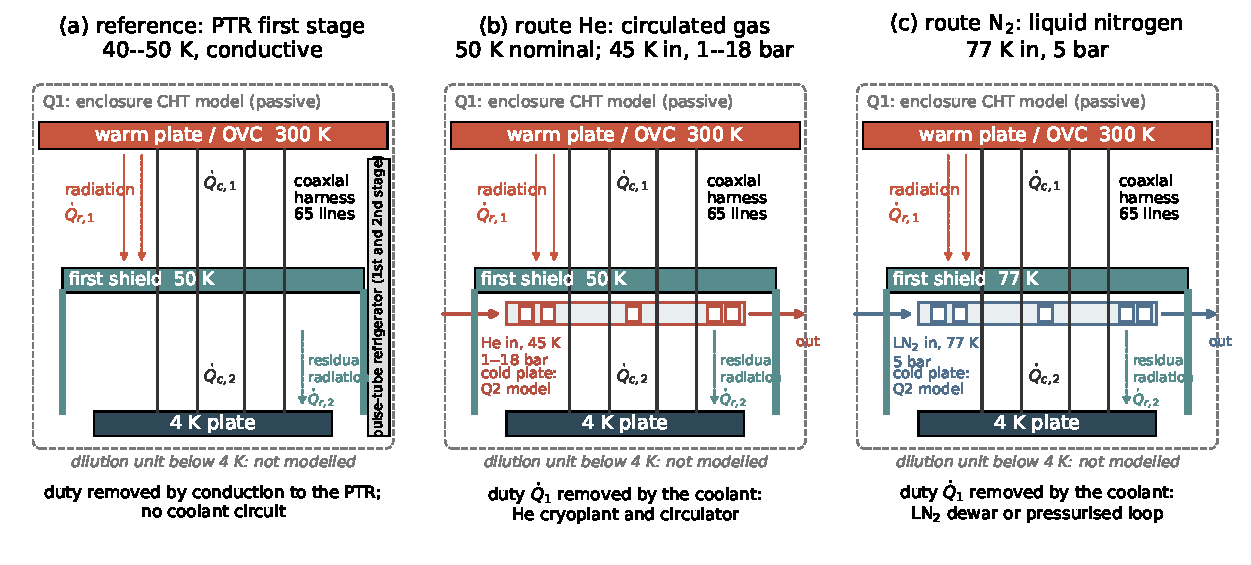
\includegraphics[width=0.95\textheight]{fig1_schematic}
\caption{The three first-shield cooling routes and the two models, drawn for the cryostat
class studied: a 300\,K warm plate and outer vacuum can, a first shield at 50 or 77\,K and a
4\,K plate, with the dilution unit or payload below 4\,K not modelled. (a)~Reference
architecture with a conductively coupled PTR first stage; (b)~circulated helium gas through a
channelled cold plate; (c)~liquid nitrogen through the same cold plate. The dashed box is the
domain of the passive enclosure CHT model (Q1); the shaded channel row is the domain of the
active cold-plate model (Q2). The loads $\dot Q_1 = \dot Q_{r,1}+\dot Q_{c,1}$ and $\dot Q_2 = \dot Q_{r,2}+\dot Q_{c,2}$
enter the work ledger (Q3), $\dot W=\sum_i\dot Q_i(T_0-T_i)/(T_i\eta_i)$, with $\eta_i=1$ (ideal)
or the measured fraction of Carnot (real).}
\label{fig:schematic}
\end{sidewaysfigure}

% =====================================================================
\section{Models and methods}
\label{sec:methods}

\subsection{Governing equations}
\label{sec:eqs}

Both models solve steady conservation equations with OpenFOAM
v2412~\cite{38-OpenFOAM2412}. In the enclosure model the inter-stage gaps are vacuum, so each
gap region carries only the radiative exchange and each solid region carries conduction with a
temperature-dependent conductivity,
\begin{equation}
\nabla\cdot\big[\kappa_{\mathrm{eff}}(T)\,\nabla T\big]=0 \quad\text{in the harness bundles},
\label{eq:solid}
\end{equation}
coupled at the bundle surfaces to the radiative flux of the enclosing gap. Radiation is
solved as a grey-diffuse radiosity system on the agglomerated boundary faces,
\begin{equation}
J_i=\varepsilon_i\sigma T_i^{4}+(1-\varepsilon_i)\sum_j F_{ij}J_j,\qquad
q_{r,i}=J_i-\sum_j F_{ij}J_j ,
\label{eq:radiosity}
\end{equation}
where $F_{ij}$ are geometric view factors computed by ray tracing between agglomerated faces
(\texttt{viewFactor} model). For two parallel grey surfaces Eq.~(\ref{eq:radiosity}) reduces to
the closed form $q_r=\sigma(T_{\mathrm{hot}}^4-T_{\mathrm{cold}}^4)/(1/\varepsilon_{\mathrm{hot}}
+1/\varepsilon_{\mathrm{cold}}-1)$~\cite{25-Bergman2017HeatTransfer}, which is used as the
verification anchor.

The cold-plate model solves the steady Reynolds-averaged (or, in the laminar range, the
plain) continuity, momentum and energy equations for a single-phase coolant,
\begin{align}
\nabla\cdot(\rho\mathbf U)&=0,\\
\nabla\cdot(\rho\mathbf U\mathbf U)&=-\nabla p+\nabla\cdot\big[(\mu+\mu_t)
(\nabla\mathbf U+\nabla\mathbf U^{\mathsf T})\big]+\rho\mathbf g,\\
\nabla\cdot(\rho\mathbf U h)&=\nabla\cdot\Big[\Big(\frac{k}{c_p}+\frac{\mu_t}{\Pr_t}\Big)\nabla h\Big],
\label{eq:energy}
\end{align}
with $\mu_t=0$ for laminar runs and $\mu_t$ from the $k$--$\omega$ shear-stress transport (SST)
model~\cite{Menter1994SST} for $\Re\ge 5000$ ($\Pr_t=0.85$). The sweep is run as pure
forced convection ($\mathbf g=0$) so that the ranking does not depend on the orientation of
the plate; the buoyancy parameter $\mathrm{Gr}/\Re^2$ is reported for every run, and four
runs with gravity acting along the heated wall quantify the mixed-convection sensitivity
(Section~\ref{sec:res-q2}). Helium is treated as an ideal gas
with variable density, $\rho=pM/(R_uT)$, because its density changes by 5--26\,\% between inlet and outlet and by up to a factor of 2 between bulk and heated wall; liquid nitrogen is treated with the Boussinesq
approximation, $\rho=\rho_0[1-\beta(T-T_0)]$, for which $\beta\Delta T\le0.05$ in every run
(largest at $\Re=500$, where the wall sits 8.7\,K above the inlet), within the first-order
range of the approximation.

\subsection{Enclosure CHT model (Q1)}
\label{sec:enclosure}

The domain is a $0.718\times0.718\times0.335$\,m section of a cryostat between the warm plate
and the first-stage cold plate (Fig.~\ref{fig:domain}; Table~\ref{tab:enclosure}). Two vacuum
gap regions (outer: outer vacuum can (OVC) to shield; inner: warm plate to cold plate and shield) and four solid
cylinders of 20\,mm diameter spanning the 0.335\,m height are meshed with a
$30\times30\times14$ background grid refined to level~2 around the cylinders
(0.2--0.4$\times10^{6}$ cells in total). Each cylinder lumps one functional family of a
cabled 65-line control harness~\cite{6-Krinner2019CryogenicSetup}: 25 drive, 25 flux, 10
readout and 5 pump lines, all of the UT-085 stainless-steel/PTFE coaxial construction. The
family is represented by an effective conductivity
\begin{equation}
\kappa_{\mathrm{eff}}(T)=\frac{n_k}{A_{\mathrm{model}}}\sum_{i}A_i\,k_i(T),
\label{eq:keff}
\end{equation}
where $n_k$ is the number of lines in the family, $A_i$ the cross-section of cable component
$i$ (outer conductor 1.585\,mm$^2$ and centre conductor 0.205\,mm$^2$ of 304 stainless steel,
polytetrafluoroethylene (PTFE) dielectric 2.001\,mm$^2$), $k_i(T)$ the NIST cryogenic conductivity fits, and
$A_{\mathrm{model}}$ the conduction cross-section of the modelled cylinder in the stage span
concerned, calibrated from the mesh so that the resolved conduction reproduces the harness integral
$n_k L^{-1}\sum_i A_i\int k_i\,\mathrm{d}T$ (Supplementary Tables~S3 and~S4 list the
areas, lengths, per-bundle targets and the fifth-order polynomial coefficients of $\kappa_{\mathrm{eff}}$ for every bundle and
stage span; fit error below 0.5\,\%; Fig.~\ref{fig:harness}). The stage-integrated conduction
is therefore fixed by the cable data by construction, and the model is credited only with its
distribution among bundles and its coupling to the radiation field, not with its total.

\begin{figure}[tbp]
\centering
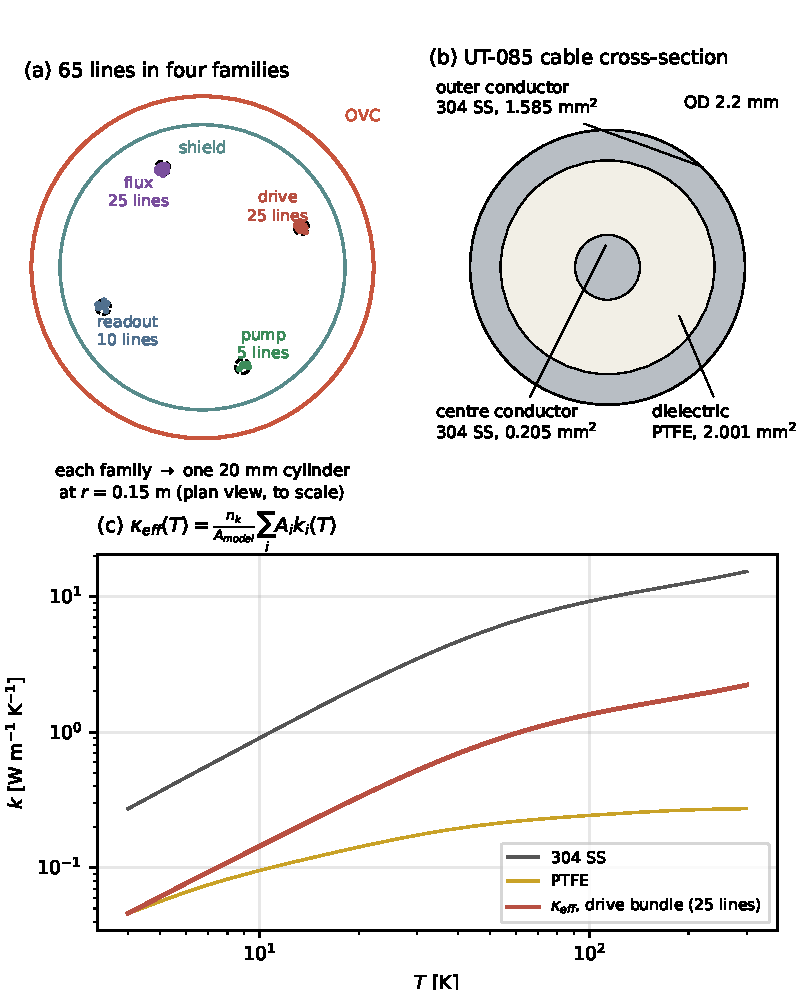
\includegraphics[width=0.9\textwidth]{figC_harness_lumping}
\caption{Harness representation: (a)~the 65 coaxial lines in four functional families, each
lumped into one 20\,mm cylinder; (b)~the UT-085 cable cross-section with the component
areas of Eq.~(\ref{eq:keff}); (c)~the component conductivities and the resulting effective
conductivity of the drive bundle.}
\label{fig:harness}
\end{figure}


\begin{table}[tbp]
\centering\small
\caption{Enclosure model: geometry, boundary conditions and numerical settings.}
\label{tab:enclosure}
\begin{tabularx}{\textwidth}{l X}
\toprule
Domain & $0.718\times0.718\times0.335$\,m; OVC and shield as snapped stereolithography (STL) surfaces; four coax
cylinders $\varnothing 20$\,mm at radius 0.15\,m \\
Regions & \texttt{domain0} (OVC--shield gap), \texttt{domain1} (warm plate--cold plate/shield gap),
\texttt{coax\_L1..L4} (solids) \\
Gas in gaps & vacuum: $p=10^{-3}$\,Pa, $g=0$, $\mu=10^{-11}$\,Pa\,s (no convection, negligible
gas conduction; the residual-gas bound is free-molecular helium at $10^{-4}$\,Pa, 24\,mW or 2.3\,\% of the harness conduction, Supplementary S1) \\
Temperatures & fixed: warm plate and OVC at $T_{\mathrm{hot}}$; shield and cold plate at
$T_{\mathrm{cold}}$; cases (300, 50), (300, 77), (50, 4), (77, 4)\,K \\
Emissivity (baseline) & warm surfaces 0.04 (polished Al); shield and cold plate 0.02
(polished Cu-plated steel); harness 0.02 \\
Emissivity (variants) & $\pm50$\,\% (0.02/0.01 and 0.06/0.03); multi-layer-insulation (MLI) equivalent 0.003 on all
first-stage surfaces \\
Radiation & \texttt{viewFactor}, grey diffuse, one band, solved every 10 iterations;
agglomeration 250 faces per patch at the coarsest level (verification at 400 and 800) \\
Harness contact & bundles fixed at $T_{\mathrm{hot}}$ at the warm cap and $T_{\mathrm{cold}}$ at the
cold cap; no contact resistance; lateral surfaces exchange by radiation only \\
Solver & \texttt{chtMultiRegionSimpleFoam}, semi-implicit method for pressure-linked equations (SIMPLE), residuals $<10^{-7}$, 2900 iterations
from a uniform initial field \\
\bottomrule
\end{tabularx}
\end{table}

\begin{figure}[tbp]
\centering
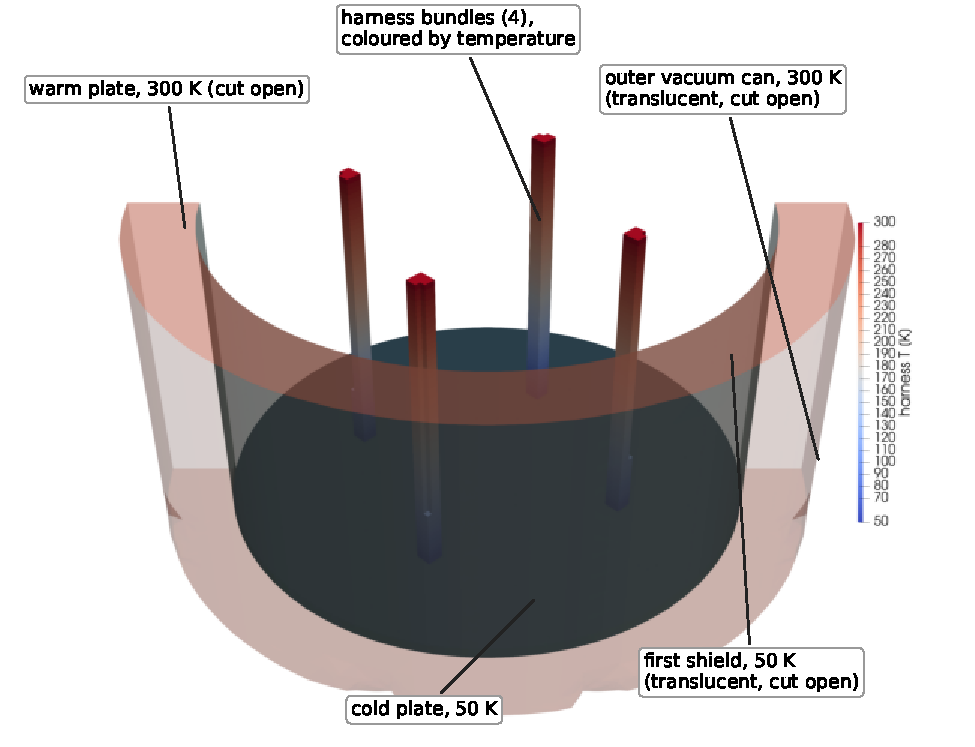
\includegraphics[width=\textwidth]{fig1_domain_v2}
\caption{Cut-away of the enclosure CHT domain for the 300\,$\to$\,50\,K case. The warm plate,
outer vacuum can and first shield are cut open on the near side; the four harness bundles,
coloured by their computed temperature, span the gap from the warm plate to the cold plate. The
vacuum gaps between the surfaces carry radiation only.}
\label{fig:domain}
\end{figure}

\paragraph{Verification and uncertainty.} Stage-integrated radiation is compared with the
parallel-plate closed form and harness conduction with the analytic integral; both agree
within the tolerances reported in Section~\ref{sec:res-q1}. Because the view-factor matrix is
built on agglomerated faces, the radiative load was recomputed at 250, 400 and 800 coarse
faces per patch and its closure $\sum_jF_{ij}$ monitored (Supplementary Table~S5). The
emissivity of polished cryogenic surfaces is uncertain by roughly a factor of
1.5~\cite{27-Ekin2006Experimental}; the $\pm50$\,\% runs give the uncertainty band carried
through the ledger. An MLI-equivalent variant with $\varepsilon=0.003$ on the first-stage surfaces
represents a 10--20 layer blanket~\cite{Shu1986MLI, 21-Weisend2016Cryostat}.

\paragraph{What the three-dimensional model adds.} For a parallel-plate enclosure with fixed
wall temperatures, the stage-integrated radiative and conductive loads are analytic, and the
CHT model must reproduce them; that agreement is the model's verification, not its result. The
model contributes what the closed forms cannot: the distribution of radiative flux over the
shield (which sets local shield temperatures once a real, finitely conductive shield is
considered), the coupling between the harness and the surrounding radiation field, the
first-stage duty that sets the cold-plate load, and the dependence of the 4\,K-stage load on
the first-stage temperature that closes the loop between the cold-plate and ledger models
(Section~\ref{sec:res-q3}). The partition of conduction among harness families follows from
the cable counts and is not claimed as a result. For the cold plate the closed forms are the fully developed duct limits and
the Gnielinski correlation; what the model adds there is the developing-flow Nusselt map
across Reynolds number and pressure, the departure of a single-wall-heated duct from the
correlations for uniformly heated ducts, and the wall-temperature distributions, including the
local maximum that sets the saturation margin, none of which a correlation
supplies (Section~\ref{sec:res-q2}).

\subsection{Cold-plate heat-exchanger model (Q2)}
\label{sec:hx}

\paragraph{Basis of comparison.} The two fluids differ in phase, temperature, density by a
factor of 800 and thermal conductivity by a factor of 3.1, so no single common basis is
neutral. Three bases are therefore reported: matched Reynolds number (same flow regime),
matched mass flow, and matched pumping power. All runs remove the same duty of 9.4\,W, the
conservative first-stage load of Section~\ref{sec:res-q1}. Helium enters at 45\,K, at 1, 5 or
18\,bar (the ITER shield loop runs at 18\,bar~\cite{Nam2014ITERThermalShield}); nitrogen enters
as a liquid at 77\,K in a 5\,bar loop, for which $T_{\mathrm{sat}}=94.0$\,K (87.9\,K at 3\,bar).
The Boussinesq solution does not depend on the loop pressure, since the 77\,K liquid properties
change by less than 0.3\,\% between 3 and 5\,bar, so one set of fields serves both pressures;
the saturation margin $T_{\mathrm{sat}}-T_{\mathrm{w,max}}$, with $T_{\mathrm{w,max}}$ the hottest
face of the heated-wall patch, is reported for every run to confirm single-phase operation. Table~\ref{tab:hx} lists the operating quantities and Fig.~\ref{fig:hxgeom} the geometry.

\begin{table}[tbp]
\centering\footnotesize
\renewcommand{\arraystretch}{1.18}
\setlength{\tabcolsep}{4pt}
\caption{Cold-plate model: geometry, coolant states, properties and numerics. Properties from
the NIST reference equations of state via CoolProp~\cite{Bell2014CoolProp}, evaluated at the
inlet state and held constant except for the helium density (ideal gas) and the nitrogen
buoyancy term.}
\label{tab:hx}
\begin{tabular}{>{\raggedright\arraybackslash}p{3.5cm} >{\raggedright\arraybackslash}p{4.4cm} >{\raggedright\arraybackslash}p{4.4cm}}
\toprule
\multicolumn{3}{l}{\textbf{Shared geometry and duty}} \\
\midrule
Channels & \multicolumn{2}{>{\raggedright\arraybackslash}p{9.4cm}}{five parallel square ducts, one wall heated} \\
Dimensions & \multicolumn{2}{>{\raggedright\arraybackslash}p{9.4cm}}{$D_{\mathrm h}=10$\,mm, $L=0.30$\,m; $A_{\mathrm{heated}}=0.015$\,m$^2$, $A_{\mathrm{cs}}=5\times10^{-4}$\,m$^2$} \\
Duty & \multicolumn{2}{>{\raggedright\arraybackslash}p{9.4cm}}{9.4\,W, uniform flux $q_{\mathrm w}=627$\,W\,m$^{-2}$ on the heated wall} \\
Mesh & \multicolumn{2}{>{\raggedright\arraybackslash}p{9.4cm}}{$180\times18\times18$ cells per duct, wall-graded (ratio 6); $2.92\times10^{5}$ cells; GCI on 86k / 292k / 984k} \\
Gravity & \multicolumn{2}{>{\raggedright\arraybackslash}p{9.4cm}}{off (forced convection); on for three sensitivity runs} \\
\midrule
 & \textbf{Helium gas} & \textbf{Liquid nitrogen} \\
\midrule
\multicolumn{3}{l}{\textit{Coolant state}} \\
Inlet temperature & 45\,K & 77\,K \\
Loop pressure & 1, 5 or 18\,bar & 5\,bar ($T_{\mathrm{sat}}=94.0$\,K; 87.9\,K at 3\,bar) \\
Phase & ideal gas, variable density & single-phase liquid (margin reported) \\
\addlinespace[3pt]
\multicolumn{3}{l}{\textit{Properties at the inlet state}} \\
Density $\rho$ [kg\,m$^{-3}$] & 0.961 / 4.80 / 17.3 at 1 / 5 / 18\,bar & 808 \\
$c_p$ [J\,kg$^{-1}$K$^{-1}$] & 5201 & 2038 \\
Viscosity $\mu$ [$\mu$Pa\,s] & 6.36 & 163.5 \\
$k$ [W\,m$^{-1}$K$^{-1}$] & 0.0467 & 0.1457 \\
Prandtl number $\Pr$ & 0.71 & 2.29 \\
$\beta$ [K$^{-1}$] & $1/T$ (ideal gas) & $5.6\times10^{-3}$ \\
\addlinespace[3pt]
\multicolumn{3}{l}{\textit{Flow range}} \\
Reynolds numbers & \multicolumn{2}{>{\raggedright\arraybackslash}p{9.4cm}}{500, 1000, 1500, 2300 (laminar); 5000, 10\,000 ($k$--$\omega$ SST)} \\
$\dot m$ at $\Re=2300$ [kg\,s$^{-1}$] & $7.31\times10^{-4}$ & $1.88\times10^{-2}$ \\
$U$ at $\Re=2300$ [m\,s$^{-1}$] & 1.52 (1\,bar); 0.084 (18\,bar) & 0.047 \\
\addlinespace[3pt]
\multicolumn{3}{l}{\textit{Numerics}} \\
Solver & \texttt{buoyantSimpleFoam} (ideal gas) & \texttt{buoyantBoussinesqSimpleFoam} \\
Convergence & residuals $<10^{-6}$ & residuals $<10^{-7}$ \\
Energy closure & \multicolumn{2}{>{\raggedright\arraybackslash}p{9.4cm}}{per run; $<0.2$\,\% for every forced-convection case} \\
\bottomrule
\end{tabular}
\end{table}

\paragraph{Property reference state.} The helium transport properties are the NIST values at
50\,K and 1\,bar, $\mu=6.36\,\mu$Pa\,s and $k=0.0467$\,W\,m$^{-1}$\,K$^{-1}$
($\mathrm{Pr}=0.709$), held constant in each run with the density from the ideal-gas law; the
inlet is 45\,K and the wall reaches 106\,K at $\Re=500$, over which range $\mu$ and $k$ both
rise by about 65\,\%. Two
sensitivity runs with cubic $\mu(T)$ and $k(T)$ fitted to the NIST data
over 40--100\,K (fit error below 0.05\,\%) are reported in Section~\ref{sec:res-q2-verif}. The
reference state matters: gas properties taken 35\,K too cold would understate $h$ by a factor
of about 2.5.


\begin{figure}[tbp]
\centering
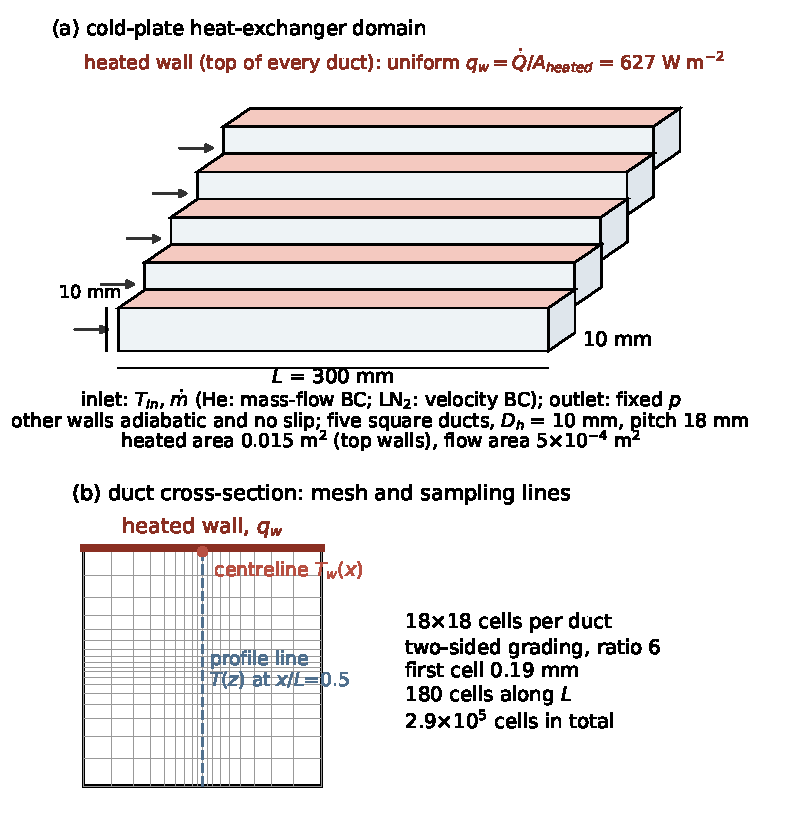
\includegraphics[width=\textwidth]{figB_coldplate_geometry}
\caption{Cold-plate heat-exchanger model: (a)~the five heated square ducts with boundary
conditions and dimensions; (b)~the graded duct cross-section with the two sampling lines
used for the wall-temperature profiles.}
\label{fig:hxgeom}
\end{figure}

\paragraph{Metrics.} The heat-transfer coefficient is
$h=\dot Q/[A_{\mathrm{heated}}(T_{\mathrm w}-T_{\mathrm b})]$ with $T_{\mathrm w}$ the
area-averaged heated-wall temperature and $T_{\mathrm b}$ the mean of the inlet and the
mass-flux-weighted outlet temperature; $\Nu=hD_{\mathrm h}/k$; the Darcy friction factor
$f=2\Delta p D_{\mathrm h}/(\rho U^2L)$; pumping power $\dot W_{\mathrm p}=\dot m\Delta p/\rho$;
NTU $=hA/(\dot m c_p)$ and $\varepsilon=1-\mathrm e^{-\mathrm{NTU}}$~\cite{42-KaysLondon1984}; the
Mouromtseff number $\mathrm{Mo}=k^{0.6}\rho^{0.8}c_p^{0.4}\mu^{-0.4}$~\cite{40-Mouromtseff1942}. Laminar results are checked against the
fully developed square-duct limits for one heated and three adiabatic walls,
$\Nu_\infty\approx2.71$~\cite{39-ShahLondon1978} (a finite-difference solution of the fully
developed problem on the present cross-section gives 2.69; the four-wall value is 3.61) and
$f\Re=56.9$, and turbulent results are compared with the Gnielinski
correlation~\cite{Gnielinski1976}, which is for uniformly heated ducts and serves as a
reference rather than a benchmark. Wall temperatures are taken on the heated-wall patch
itself: its area mean, its hottest and coldest faces, and the face-value profile along the
centre row of the first channel.

\paragraph{Grid convergence.} Three systematically refined meshes (refinement ratio 1.5) were
run for both fluids at $\Re=2300$ and the discretisation uncertainty expressed as a GCI~\cite{45-Celik2008GCI} (Section~\ref{sec:res-q2}). For the turbulent runs the
first-cell $y^+$ on the graded mesh averages 2.5--5.6 with a maximum of 9.5, within the range handled
by the low-Reynolds wall treatment of the SST model.

\subsection{Work ledger (Q3)}
\label{sec:ledger-method}

A load $\dot Q_i$ absorbed at $T_i$ and rejected at $T_0=300$\,K costs
\begin{equation}
\dot W_i=\frac{\dot Q_i}{\eta_i}\,\frac{T_0-T_i}{T_i},
\label{eq:ledger}
\end{equation}
where $\eta_i$ is the stage efficiency as a fraction of Carnot. The ideal ledger sets
$\eta_i=1$: the multiplier is 5.0 at 50\,K, 2.9 at 77\,K and 74 at 4\,K. The real ledger uses
published hardware. A commercial two-stage PTR (Cryomech PT415) delivers 1.5\,W at 4.2\,K together with 40\,W at
45\,K for 10.7\,kW of input~\cite{Bluefors2026PT415}, so the two stages together return
3.1\,\% of their combined Carnot work. A single machine cannot separate the two stage
efficiencies, so the ledger takes them from Radebaugh's survey~\cite{Radebaugh2009Cryocoolers}:
$\eta_2=0.008$--0.015 at 4\,K and $\eta_1=0.10$--0.15 at 45--80\,K (Supplementary S3). These
ranges are consistent with the PT415: at their midpoints the two stages would need 11.4\,kW,
within 7\,\% of the rated input. Liquid nitrogen
carries 199\,kJ\,kg$^{-1}$ of latent heat at 1\,bar; its ideal production work is
0.213\,kWh\,kg$^{-1}$~\cite{BarronNellis2016Cryogenic} and real air-separation plants need
0.5--0.7\,kWh\,kg$^{-1}$~\cite{Karabuga2018N2Liquefaction}, an exergy efficiency
$\eta_{\mathrm{N_2}}\approx0.3$--0.4. The 4\,K stage of the nitrogen route is still served by a
cryocooler, so its $\eta_2$ is the same in both routes. The ranges above are propagated as
bands.

% =====================================================================
\section{Results Q1: the passive penalty of a 77\,K shield}
\label{sec:res-q1}

\subsection{Radiation verification and the view-factor closure}
\label{sec:res-q1-rad}

The first-stage radiative load computed with the view-factor matrix as generated does not
converge under agglomeration refinement: 9.46, 8.41, 6.49 and 3.26\,W at 60, 250, 400 and
800 coarse faces per patch, against 7.07\,W from the parallel-plate closed form
(Fig.~\ref{fig:radsweep}). The cause is closure. In a closed enclosure every row of the
view-factor matrix must sum to one; the generated rows sum to between 0.50 and 1.13 (mean
0.97--1.01), and finer agglomeration worsens the scatter. With emissivities of 0.02--0.04 the
radiosity is reflected of order $1/\varepsilon$ times before absorption, so a per-reflection
leak of a few per cent compounds into a load error of tens of per cent. Normalising each row
to unity removes the artefact: at the production level of 250 faces the 300\,$\to$\,50\,K load
becomes 7.36\,W (4.1\,\% above the closed form), the 300\,$\to$\,77\,K load 7.34\,W (4.2\,\%),
and the two 4\,K-stage loads 3.16 and 17.8\,mW (0.5\,\% above 3.15 and 17.7\,mW). The
normalised load converges under refinement, 7.36, 7.32 and 7.27\,W at 250, 400 and 800 faces,
so the remaining 3--4\,\% combines the geometric departure of the real enclosure, with its
harness penetrations, from the parallel-plate idealisation with residual agglomeration error.
All loads below are the row-normalised values; the unnormalised production values are kept
as an upper band. Normalisation enforces closure, not reciprocity $A_iF_{ij}=A_jF_{ji}$; the
least-squares rectification procedures compared by Taylor and
Luck~\cite{TaylorLuck1995VFRectification} enforce both and would be the next refinement. Two
residuals quantify what it leaves: the net radiative power summed over every surface of a
closed region, which must vanish, is 1.5\,W for the generated matrix at 400 faces and 14\,W at
800, against 0.10, 0.13 and 0.36\,W (1.3, 1.8 and 4.9\,\% of the load) for the normalised
matrices at 250, 400 and 800 faces; and the area-weighted reciprocity error
$\sum|A_iF_{ij}-A_jF_{ji}|/\sum A_iF_{ij}$, with coarse-face areas rebuilt from the mesh
(\texttt{reciprocity.py}), is 3.9, 5.5 and 12.6\,\% at the same levels (outer gap region).
Both grow with refinement, which is why the production level is 250 faces and why the
3--4\,\% gap to the closed form is reported as the accuracy of the method.

\begin{figure}[tbp]
\centering
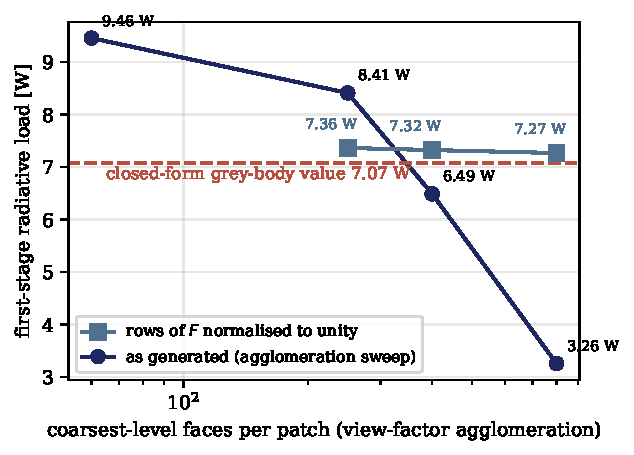
\includegraphics[width=0.7\textwidth]{fig3_radiation_sweep}
\caption{First-stage radiative load (300\,$\to$\,50\,K) against the view-factor
agglomeration level with the matrix as generated (circles) and with its rows normalised to
unity (squares), compared with the closed-form grey-body value. The monotonic collapse of the
generated matrix under refinement is a closure artefact amplified by the low emissivities;
the normalised load converges toward the closed form.}
\label{fig:radsweep}
\end{figure}

\subsection{Stage loads and mechanism split}
\label{sec:res-q1-loads}

At the first stage radiation dominates and the shield temperature barely matters
(Table~\ref{tab:loads}, Fig.~\ref{fig:loads}). The radiative flux scales with
$T_{\mathrm{hot}}^4-T_{\mathrm{cold}}^4$ and $300^4$ dwarfs both $50^4$ and $77^4$, so the
77\,K shield intercepts 99.6\,\% of what the 50\,K shield intercepts. Harness conduction
falls with the smaller span, 962 against 1029\,mW. The first-stage loads are 8.39\,W
(50\,K) and 8.30\,W (77\,K); the emissivity band of $\pm50$\,\% moves them between 6.5 and
12.5\,W but leaves the 1\,\% difference between routes unchanged. The conservative production
value of 9.4\,W is used as the cold-plate duty in Section~\ref{sec:res-q2}.

At the 4\,K stage the picture inverts. Residual radiation rises by the factor
$(77^4-4^4)/(50^4-4^4)=5.6$, but from a base of 3\,mW; harness conduction rises by the factor
2.31 from a base of 70\,mW. The 77\,K route therefore delivers 106\,mW more to the 4\,K plate:
92\,mW of conduction and 15\,mW of radiation, 86\,\% conductive. Through the ideal 4\,K
multiplier of 74 this is 7.9\,W of room-temperature power, 6.8\,W of it from the harness.
Every stage-integrated ratio agrees with its closed form to better than 0.5\,\%.

The MLI-equivalent shield ($\varepsilon=0.003$ on the first-stage surfaces) cuts the first-stage
radiation to 1.69\,W (50\,K) and 1.68\,W (77\,K) with the row-normalised matrix (closed form
1.47 and 1.46\,W; the unnormalised production matrix gives 1.81\,W on either route, the same
$+23$\,\% closure bias as at the bare-shield level), so the first-stage loads fall to 2.72 and
2.65\,W, with conduction's share rising to 36--38\,\%. The 4\,K-stage loads are unaffected. This variant is the one that
changes the ledger verdict in Section~\ref{sec:res-q3}.

\begin{table}[tbp]
\centering\small
\caption{Stage loads by mechanism (row-normalised view factors; closed-form value in
parentheses), with the unnormalised production value and the $\pm50$\,\% emissivity band as
upper and lower bounds.}
\label{tab:loads}
\footnotesize\setlength{\tabcolsep}{3pt}
\begin{tabularx}{\textwidth}{>{\raggedright\arraybackslash}p{2.35cm} r r r r >{\centering\arraybackslash}p{1.55cm}}
\toprule
Case & Radiation & Conduction & Total & Prod. & $\varepsilon\pm50\,\%$ [W] \\
\midrule
300\,$\to$\,50\,K & 7.36 W (7.07) & 1.029 W (1.029) & 8.39 W & 9.44 W & 6.5--12.5 \\
300\,$\to$\,77\,K & 7.34 W (7.04) & 0.962 W (0.962) & 8.30 W & 9.35 W & 6.4--12.4 \\
50\,$\to$\,4\,K & 3.16 mW (3.15) & 70.3 mW (70.3) & 73.5 mW & 75.6 mW & -- \\
77\,$\to$\,4\,K & 17.8 mW (17.7) & 162.1 mW (162.1) & 179.9 mW & 191.8 mW & -- \\
300\,$\to$\,50\,K MLI & 1.69 W (1.47) & 1.029 W & 2.72 W & 2.84 W & -- \\
300\,$\to$\,77\,K MLI & 1.68 W (1.46) & 0.962 W & 2.65 W & 2.77 W & -- \\
\bottomrule
\end{tabularx}
\end{table}

\begin{figure}[tbp]
\centering
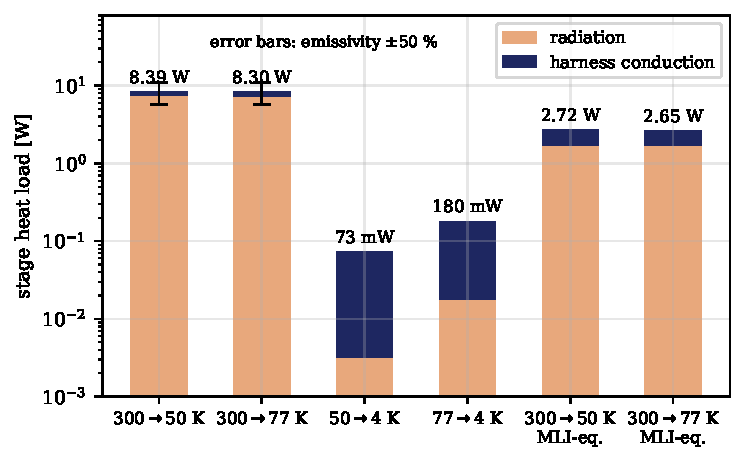
\includegraphics[width=0.85\textwidth]{fig2_cascade_loads}
\caption{Stage loads for the four enclosure cases and the two MLI-equivalent variants
(row-normalised view factors, the values used in the text), decomposed by mechanism, with the
$\pm50$\,\% emissivity band.
The first stage is radiation-dominated and nearly identical between routes; the 4\,K stage
is conduction-dominated and is where the routes diverge.}
\label{fig:loads}
\end{figure}

\subsection{Spatial distribution}
\label{sec:res-q1-spatial}

The view-factor solution concentrates the radiative flux on the shield regions with a direct
line of sight to the OVC (8.2--10.8\,W\,m$^{-2}$ across the shield) and leaves the harness
penetrations cooler (Fig.~\ref{fig:fields}). Conduction is shared among the bundles in the ratio
of their line counts: on the 77\,$\to$\,4\,K span the drive and flux families deliver 125 of
the 162\,mW. These two bundles are the targets for any intermediate heat sink, and the
harness conduction integral, not the cryogen, is the lever on the 4\,K-stage penalty.

\begin{figure}[tbp]
\centering
\begin{minipage}{0.49\textwidth}\centering
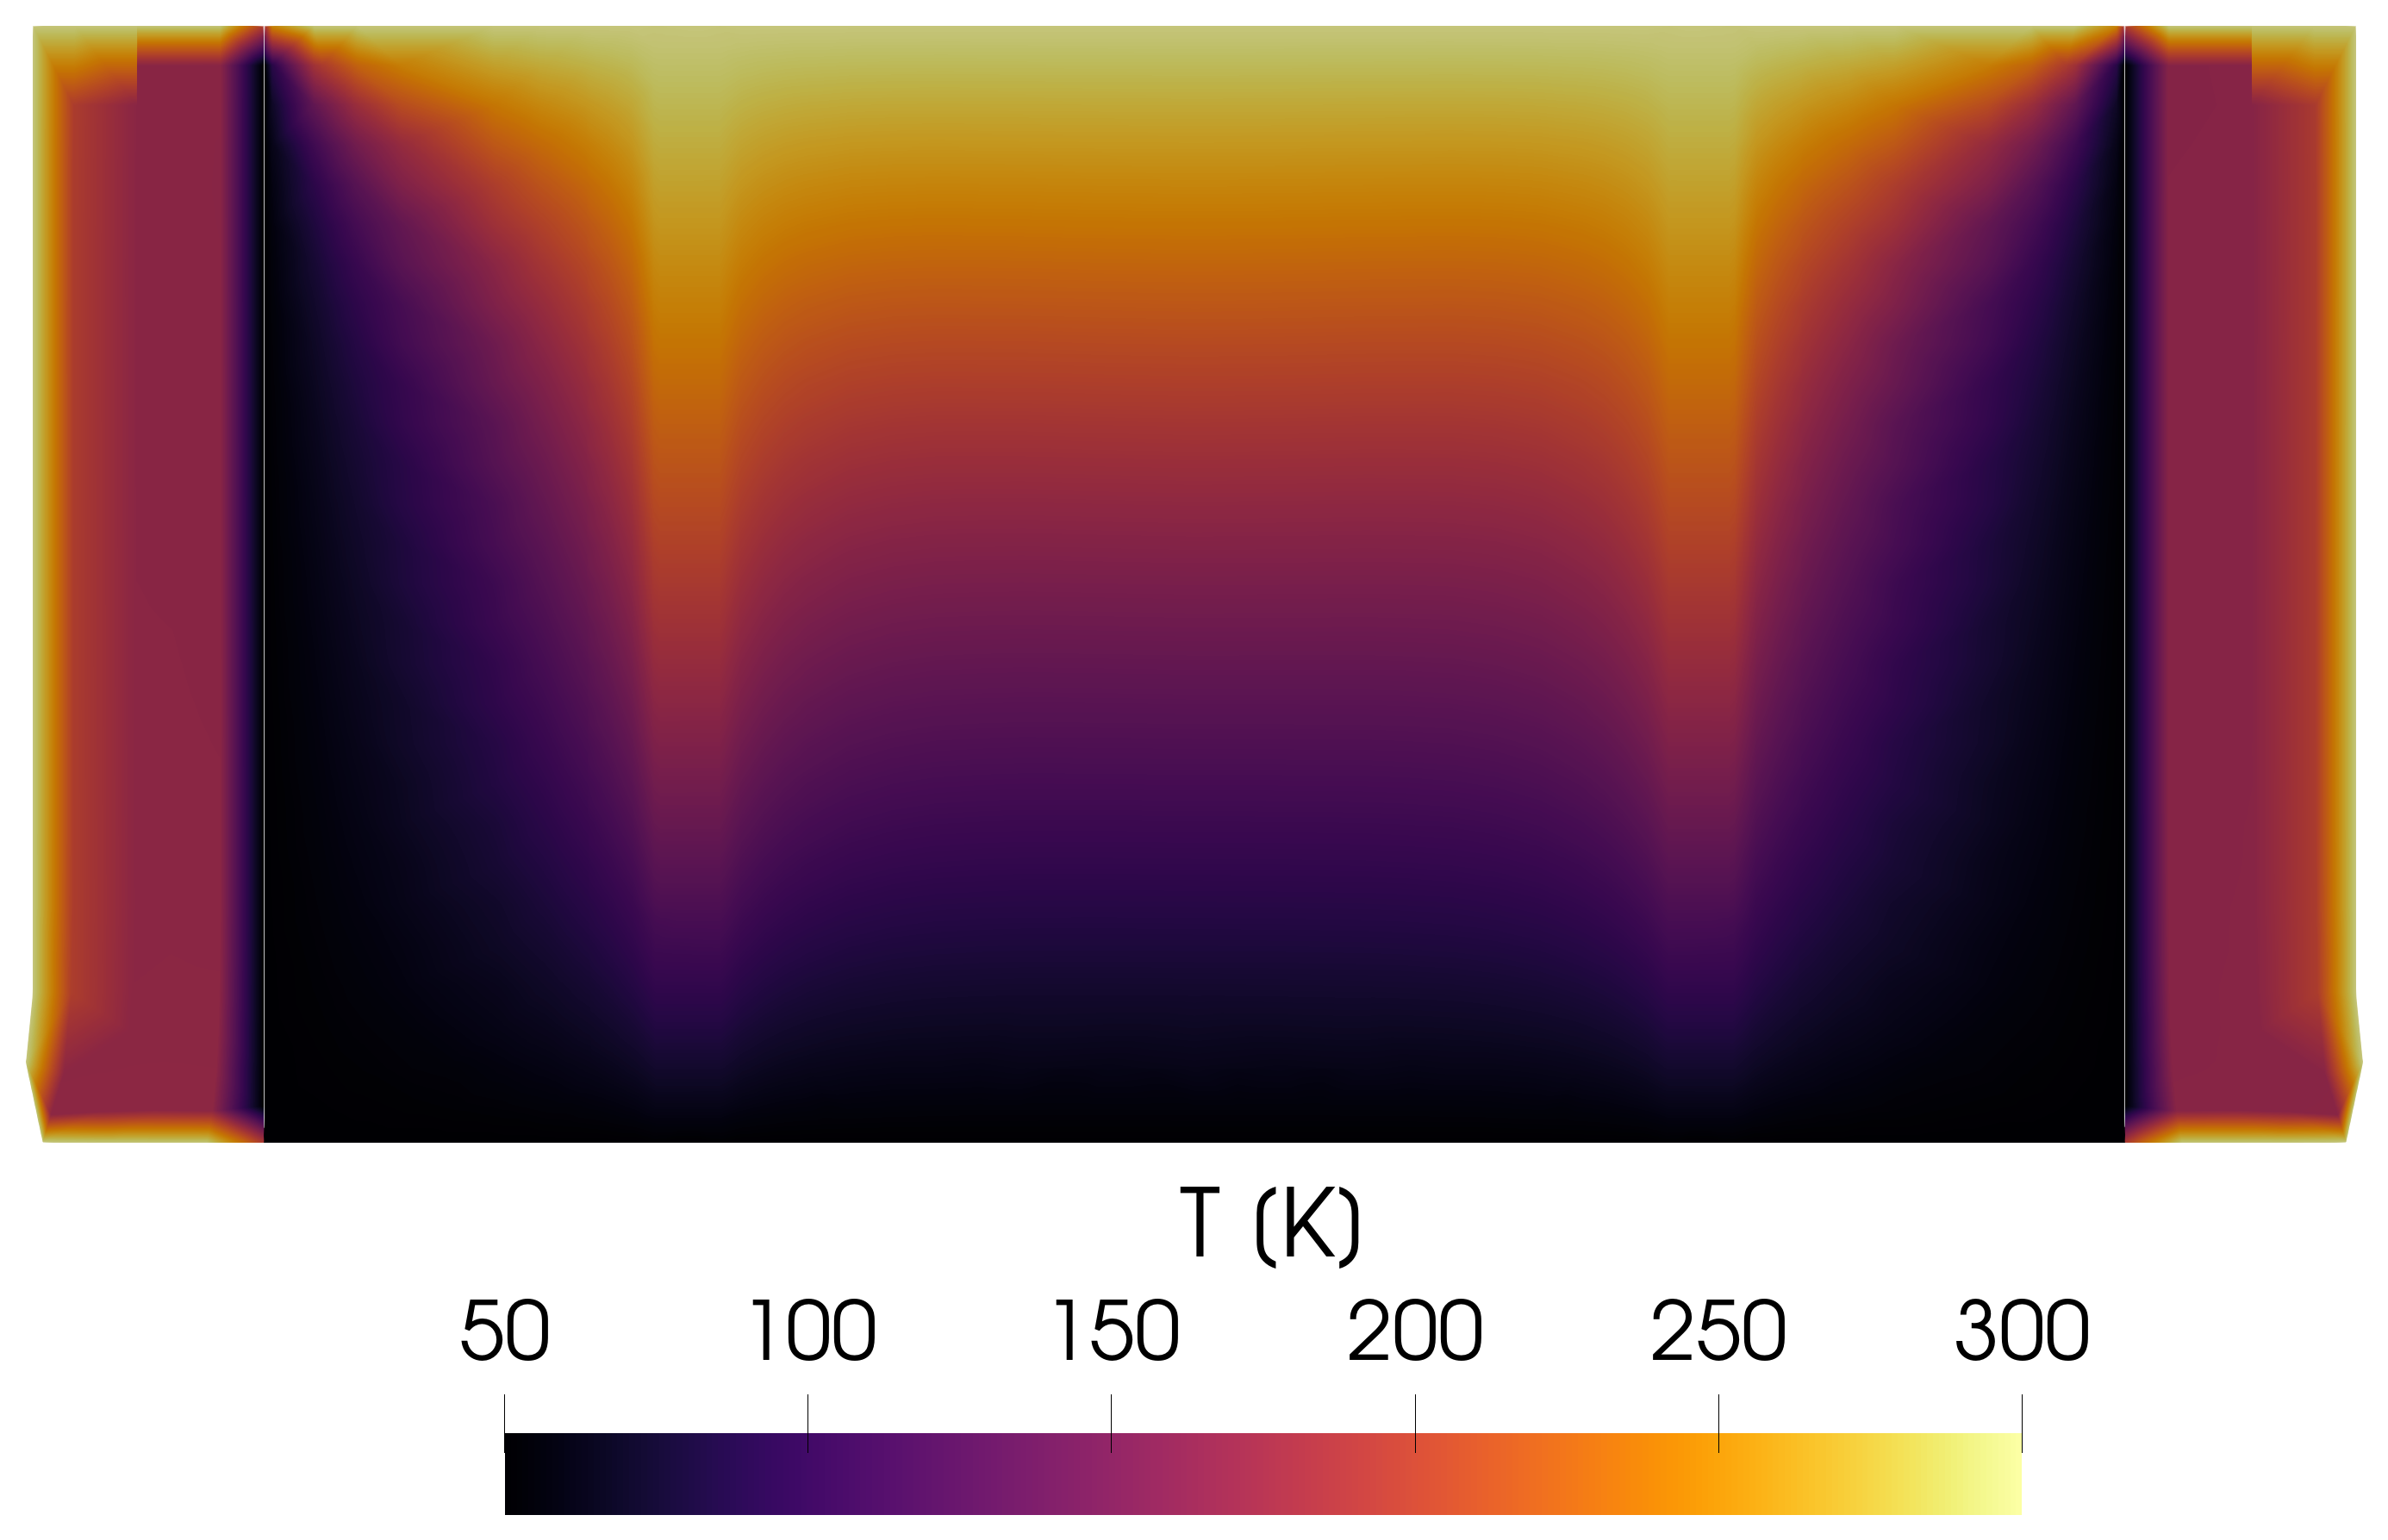
\includegraphics[width=\textwidth]{fig7a_T_midplane.png}\\ (a)\end{minipage}\hfill
\begin{minipage}{0.49\textwidth}\centering
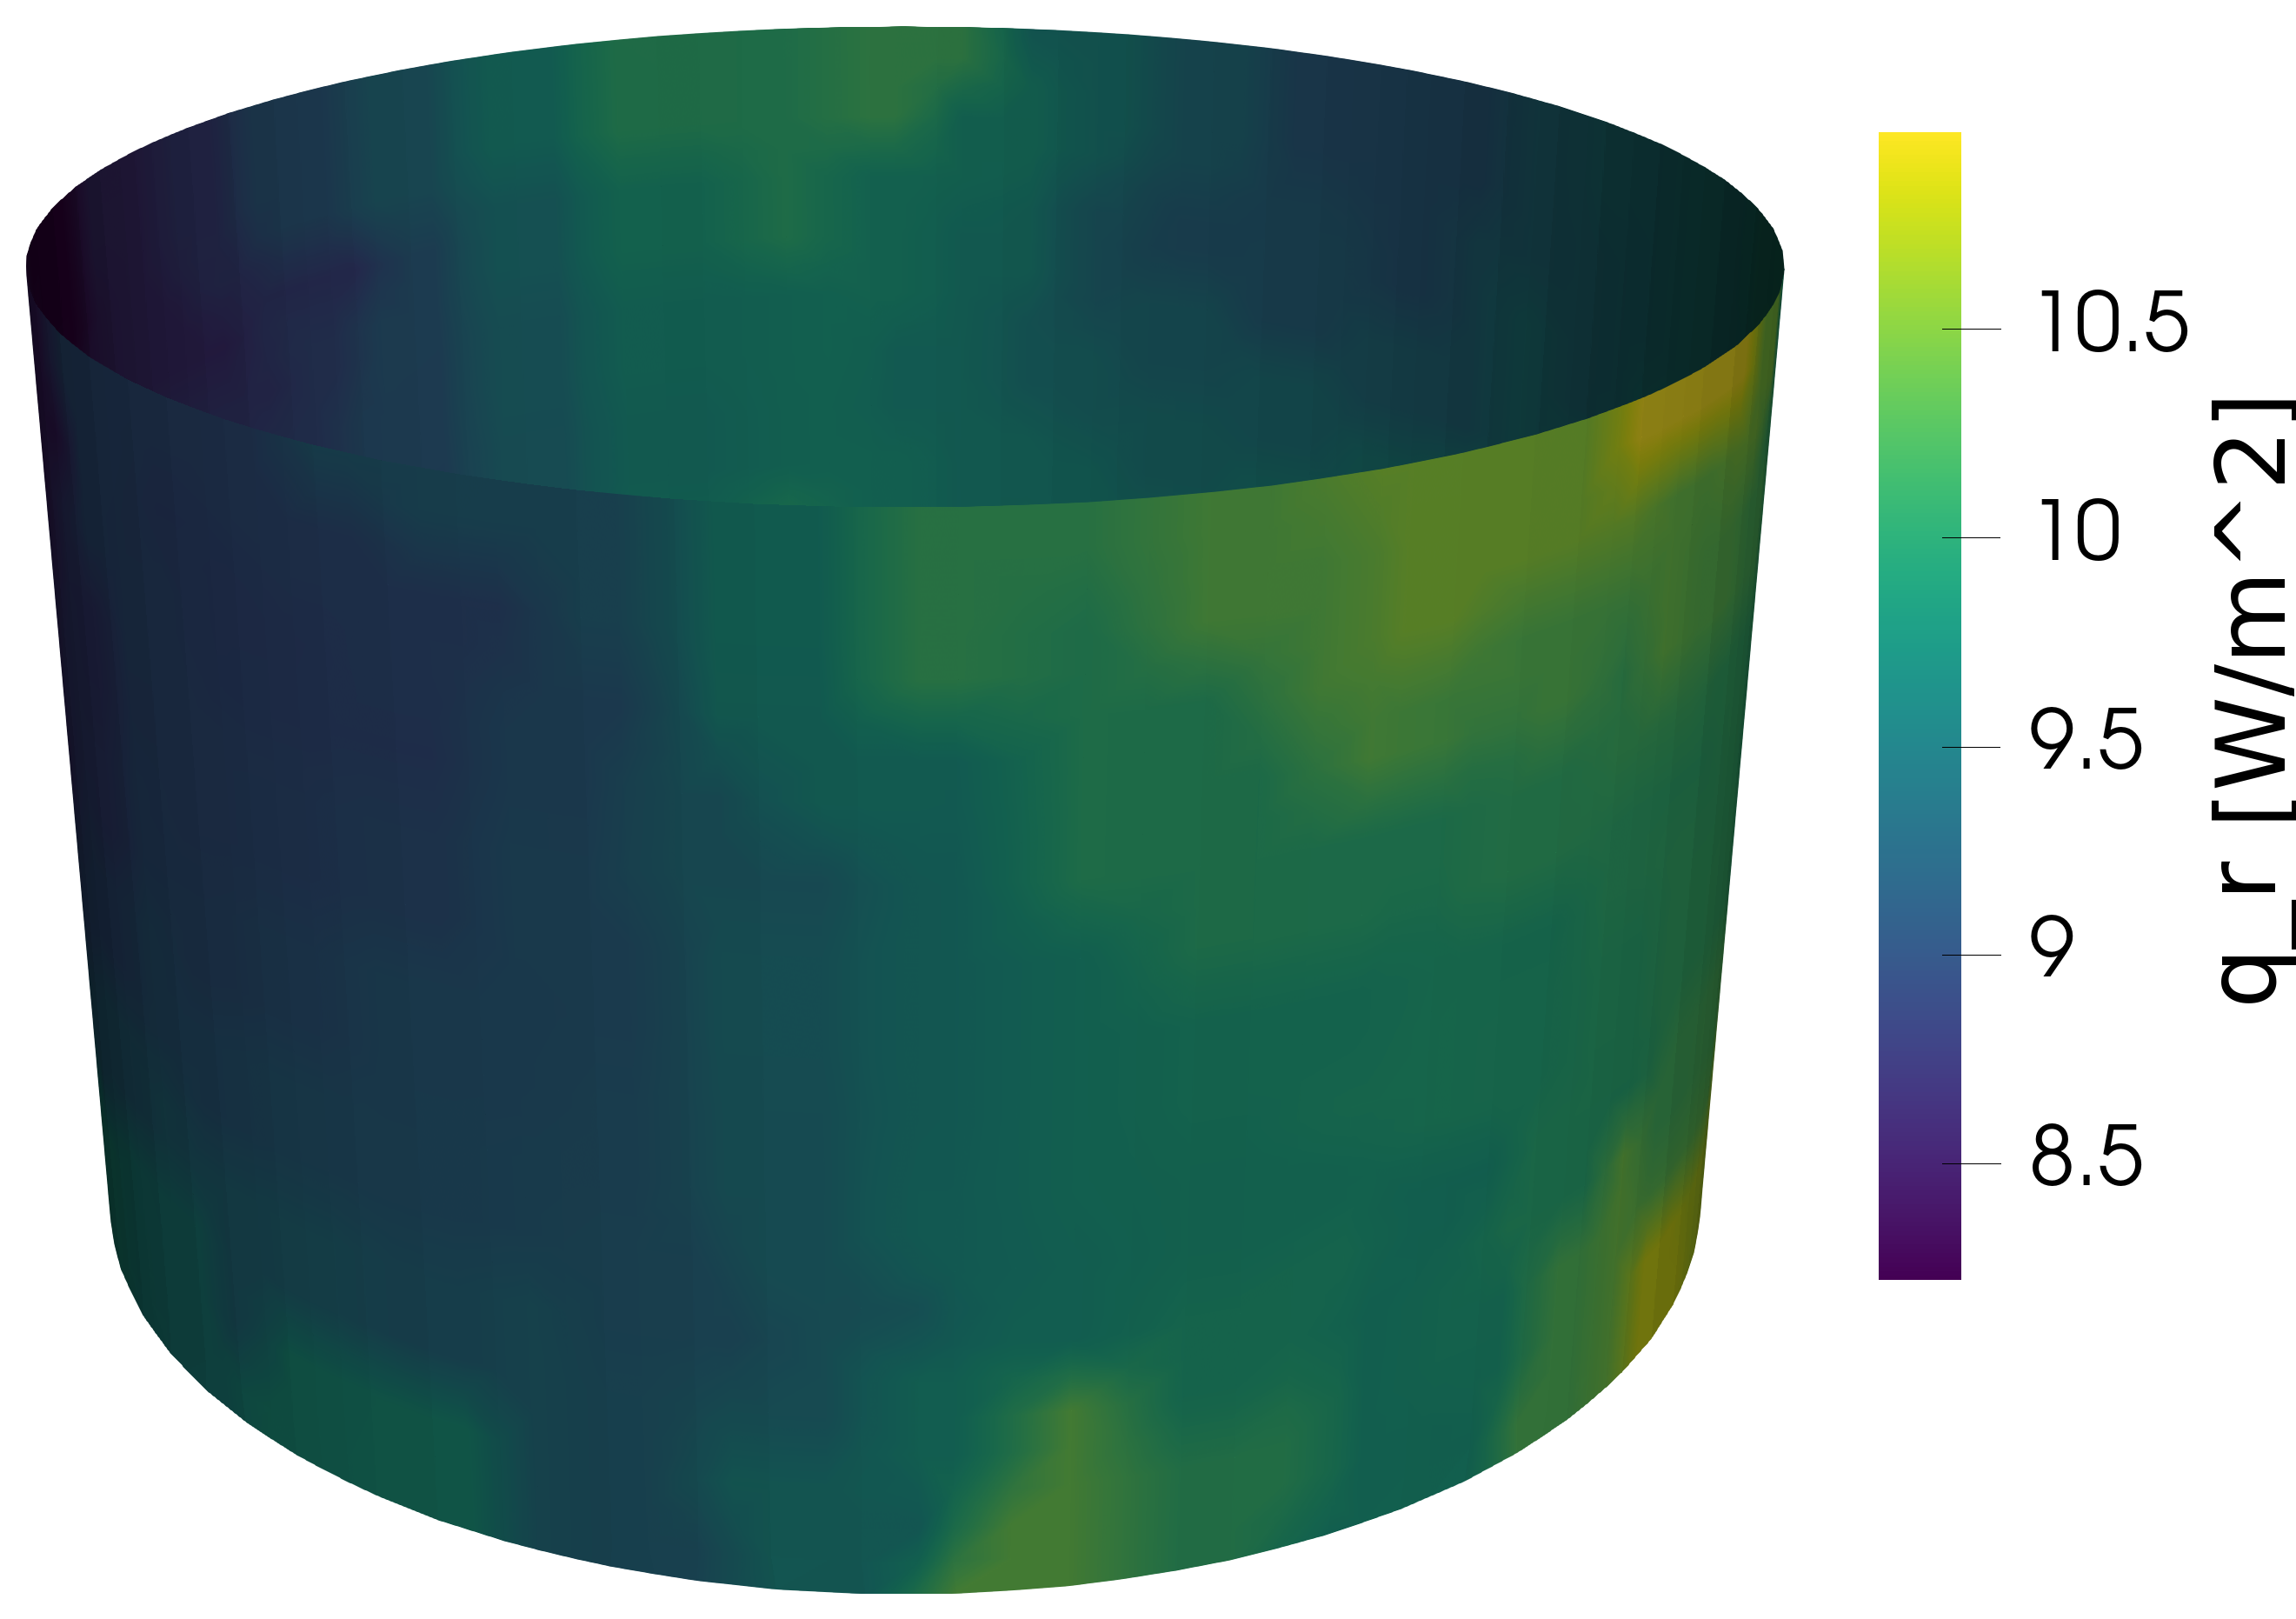
\includegraphics[width=\textwidth]{fig7b_qr_shield.png}\\ (b)\end{minipage}
\caption{(a)~Mid-plane temperature and (b)~shield radiative-flux map of the 300\,$\to$\,50\,K
case.}
\label{fig:fields}
\end{figure}

% =====================================================================
\section{Results Q2: helium gas versus liquid nitrogen in the cold plate}
\label{sec:res-q2}

\subsection{Verification}
\label{sec:res-q2-verif}

Every forced-convection run closes its energy balance, wall heat input against
mass-flux-weighted enthalpy rise, to within 0.2\,\% (Supplementary Table~S7). At $\Re=500$ the
helium flow is thermally developing over the first 59\,\% of the channel ($L_{\mathrm t}/L=0.59$) and returns
$\Nu=3.66$, 35\,\% above the fully developed limit of 2.71 for a square duct heated on one
wall~\cite{39-ShahLondon1978}, the excess being the developing-length contribution; every other
laminar run has a longer development length ($L_{\mathrm t}/L$ up to 8.8 for nitrogen) and lies
further above the limit, as it must. The three-grid
studies (Table~\ref{tab:gci}) converge monotonically for both fluids: the production-mesh
grid convergence index is 0.7\,\% ($\Nu$) and 2.5\,\% ($f$) for helium and 2.2\,\% and
1.6\,\% for nitrogen. In the turbulent runs the first-cell $y^+$ on the heated wall averages
2.5--5.6 with a maximum of 9.5, within the low-Reynolds treatment of the SST model. Nitrogen's
turbulent Nusselt numbers lie 8--9\,\% below the Gnielinski correlation~\cite{Gnielinski1976}
and helium's 28--32\,\% below it. The correlation is for a duct heated on all walls; in the
laminar limit one heated wall lowers $\Nu$ by 25\,\% (2.71 against 3.61), and the larger
deficit of the low-Prandtl gas, whose thermal layer fills the duct, is consistent with that
boundary condition but is not separately verified here, so the correlation is a reference,
not a benchmark, for these runs.

\paragraph{Property sensitivity.} Two helium runs at 1\,bar, $\Re=500$ and 2300, were repeated
with cubic $\mu(T)$ and $k(T)$ fitted to the NIST data over 40--100\,K (Section~\ref{sec:hx})
and a heat-flux wall condition using the local conductivity (delivered 9.399\,W, closure
0.01\,\%). Because $k$ rises with temperature, the hot near-wall gas conducts better than at
the 50\,K reference: at $\Re=500$ the Nusselt number rises from 3.66 to 4.16 (+14\,\%), the
plate mean falls from 87.4 to 83.0\,K and the hottest face from 106.1 to 97.3\,K, while the
friction factor and pumping power rise by 5\,\%; at $\Re=2300$ the changes are +5\,\% in
$\Nu$, $-1.0$\,K in the mean and $-2.9$\,K in the hottest face (79.7 to 76.9\,K). The 0.5\,K
by which that face clears 77.4\,K is within the uncertainty of the quantity (the three-grid
study moves it by 0.17\,K; the property fits and constant $c_p$ add a few tenths), so the
hottest-face optimum is stated as a range, $\Re\approx2300$ to 5000 and a pumping-power ratio
of 4 to 30. The constant-property results are conservative toward helium by up to 14\,\% in
$h$ at the lowest Reynolds number and 5\,\% at the design point; the rankings below are not
affected. Both runs are listed in Supplementary Table~S7.

\begin{table}[tbp]
\centering\small
\setlength{\tabcolsep}{4pt}\footnotesize
\caption{Grid convergence at $\Re=2300$ (Celik et al.~\cite{45-Celik2008GCI}; meshes of
86k, 292k and 984k cells, refinement ratio 1.5). The production mesh is the medium one.}
\label{tab:gci}
\begin{tabular}{l l r r r r r r}
\toprule
Fluid & Quantity & Coarse & Medium & Fine & $p$ & Extrapolated & GCI$_{\mathrm{medium}}$ \\
\midrule
He (1 bar) & $\Nu$ & 6.439 & 6.449 & 6.457 & 0.64 & 6.49 & 0.7\,\% \\
 & $f$ & 0.0632 & 0.0642 & 0.0647 & 1.40 & 0.0655 & 2.5\,\% \\
\LNtwo\ (3 bar) & $\Nu$ & 10.51 & 10.44 & 10.38 & 0.87 & 10.26 & 2.2\,\% \\
 & $f$ & 0.0592 & 0.0599 & 0.0603 & 1.71 & 0.0607 & 1.6\,\% \\
\bottomrule
\end{tabular}
\end{table}

\subsection{Operating maps}
\label{sec:res-q2-maps}

Figure~\ref{fig:maps} maps the two coolants over $\Re=500$--$10^4$ at the fixed 9.4\,W duty.
Nitrogen's heat-transfer coefficient exceeds helium's by 4.9--5.1 times in the laminar range
and 6.2--6.3 in the turbulent range; the laminar ratio is the conductivity ratio of 3.1 times
the ratio of developing-flow Nusselt numbers, which favours the high-Prandtl liquid. The
consequence for the plate is stark. At atmospheric pressure the helium-cooled wall averages
87\,K at $\Re=500$ and 67\,K at $\Re=2300$, with hottest faces at the channel outlet of 106
and 80\,K (Fig.~\ref{fig:maps}d). The plate mean falls below 77\,K above $\Re\approx970$, the
hottest face only in turbulent flow at $\Re=5000$ (61\,K maximum, 55\,K mean), and the
nominal 50\,K is approached only at $\Re=10^4$ and 65\,mW of pumping power (50.3\,K mean,
54.3\,K maximum). The nitrogen-cooled wall stays between 78 and 85\,K in the mean and below
89.2\,K at its hottest face; its saturation margin at 5\,bar is 4.8\,K at $\Re=500$, 9.9\,K at
2300 and 15.4\,K at $10^4$. At 3\,bar the $\Re=500$ run would exceed saturation locally (89.2
against 87.9\,K), and at 1\,bar every run would exceed 77.4\,K, so a pressurised or subcooled
loop is a requirement, not a refinement.

\begin{figure}[tbp]
\centering
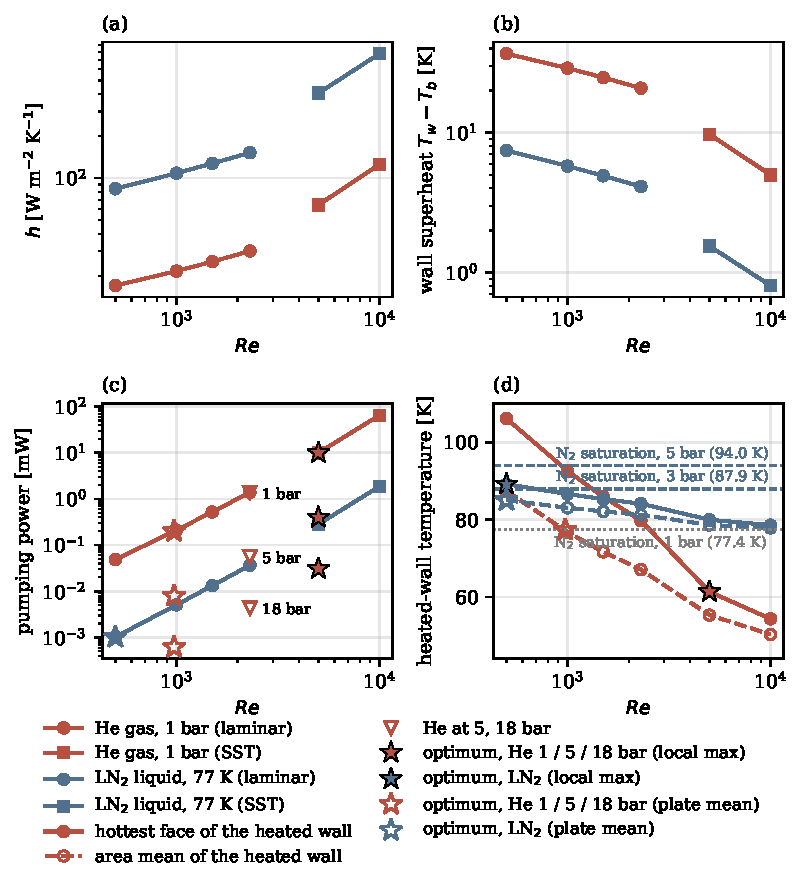
\includegraphics[width=\textwidth]{fig5_operating_maps}
\caption{Operating maps at 9.4\,W duty: (a)~heat-transfer coefficient, (b)~wall superheat,
(c)~pumping power with the helium pressure series at $\Re=2300$, and (d)~heated-wall
temperature, hottest face (filled) and area mean (open), with the nitrogen saturation
temperatures at 1, 3 and 5\,bar. Circles: laminar; squares: $k$--$\omega$ SST; stars: each
fluid's optimum, the minimum pumping power at which the wall temperature meets its limit
(77.4\,K for helium, 92.0\,K for nitrogen), filled for the hottest-face criterion and open
for the plate-mean criterion.}
\label{fig:maps}
\end{figure}

Pumping power separates the fluids in the opposite sense once pressure enters. At 1\,bar
helium needs 38 times nitrogen's pumping power at matched Reynolds number (1.39 against
0.037\,mW at $\Re=2300$), because its mass flow is 26 times smaller but its velocity 32 times
larger. Raising the helium pressure at fixed Reynolds number leaves the mass flow, the Nusselt
number and the wall temperature unchanged to four significant figures and reduces the pumping
power as the inverse square of the density: 25.0 times at 5\,bar and 324 times at 18\,bar
(Fig.~\ref{fig:maps}c). At the 18\,bar of the ITER and DTT shield loops~\cite{Nam2014ITERThermalShield,
Barone2020DTTShield} helium's pumping power is 4.3\,$\mu$W, 8.5 times below nitrogen's; the
parallel-path gaseous-helium shields of LHD operate in the same regime~\cite{Imagawa2002LHDShield}.

\paragraph{Optimum operating points.} The second half of Q2 needs an optimum: the minimum
pumping power at which the plate meets a wall-temperature limit, 77.4\,K for helium (the
temperature a nitrogen-bath plate would hold, beyond which the 50/77\,K distinction is
forfeited) and the 5\,bar saturation temperature less a 2\,K margin, 92.0\,K, for nitrogen.
The answer depends on which wall temperature is held to the limit. If the hottest face must
comply, no laminar helium run of the constant-property sweep does: the 1\,bar curve of
Fig.~\ref{fig:maps}d stays above 79.7\,K up to $\Re=2300$, and the first compliant run is the
turbulent $\Re=5000$ case at 9.95\,mW (1\,bar), 0.40\,mW (5\,bar) and 31\,$\mu$W (18\,bar);
the laminar--turbulent gap is not interpolated. The 2.4\,K margin at $\Re=2300$ is closed by
the variable-property run of Section~\ref{sec:res-q2-verif} (76.9\,K), which would move the
optimum to $\Re\approx2300$ at 1.39\,mW or 4.3\,$\mu$W at 18\,bar. Nitrogen complies at
$\Re=500$, the lowest run, with 1.0\,$\mu$W. If the plate mean is the criterion, helium
crosses 77.4\,K at $\Re\approx970$ (0.20\,mW at 1\,bar, 0.62\,$\mu$W at 18\,bar) and nitrogen
again at $\Re=500$ (stars in Fig.~\ref{fig:maps}c,d). At their optima, pressurised helium
therefore needs 4 to 30 times nitrogen's pumping power on the hottest-face criterion and
40\,\% less on the plate-mean criterion. Both are microwatts and neither enters the ledger;
what the comparison establishes is that the 38-fold penalty of atmospheric helium at matched
$\Re$ is the cost of the wrong loop pressure, not a property of the gas, and that a helium
plate must be checked against its hottest face, 13\,K above the mean at $\Re=2300$.

\subsection{Wall-temperature distributions}
\label{sec:res-q2-walls}

Figure~\ref{fig:profiles} gives the heated-wall temperature along the centre row of the first
channel, read from the wall faces themselves, and the cross-channel profile at mid-length.
Along the wall the temperature rise grows as $x^{1/3}$ in the developing region and then
linearly; at the outlet the helium wall sits 30\,K above its inlet at $\Re=2300$ and 58\,K at
$\Re=500$, nitrogen 5.5 and 10.5\,K, and the hottest faces of the patch, near the duct side
walls at the outlet where the velocity is lowest, are a further 4.8\,K (helium) and 1.6\,K
(nitrogen) warmer at $\Re=2300$. Across the channel the helium thermal layer at
$\Re=500$ fills the duct, whereas nitrogen's occupies the near-wall 30\,\% even at $\Re=500$.
This is the geometric origin of the heat-transfer ratio and of the plate temperatures in
Fig.~\ref{fig:maps}d.

\begin{figure}[tbp]
\centering
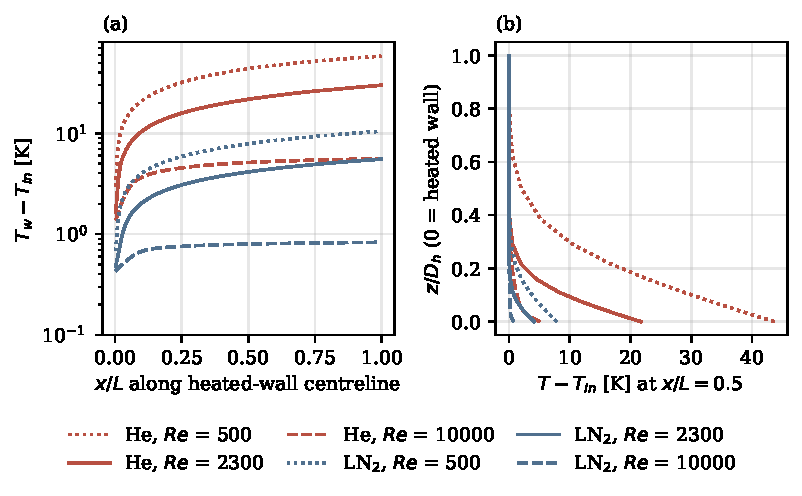
\includegraphics[width=\textwidth]{fig6_wall_profiles}
\caption{(a)~Heated-wall centreline temperature rise above the inlet and (b)~cross-channel
temperature profile at $x/L=0.5$ for both fluids at $\Re=500$, 2300 and $10^4$.}
\label{fig:profiles}
\end{figure}

\subsection{Ranking on three bases}
\label{sec:res-q2-bases}

Table~\ref{tab:design} collects the design point and Fig.~\ref{fig:pareto} the trade-off
between wall superheat and pumping power. At matched Reynolds number nitrogen wins heat
transfer by a factor of 5 and pumping power by 38; the effectiveness--NTU pair favours helium
(0.11 against 0.06), a capacity-rate artefact of the gas's small $\dot m c_p$ that says
nothing about how cold the plate is. At matched mass flow nitrogen's Reynolds number would
fall to about 90, below the sweep; the one-wall limit $\Nu_\infty\approx2.71$ bounds its
heat-transfer coefficient from below at about 40\,W\,m$^{-2}$K$^{-1}$, 1.3 times helium's at
$\Re=2300$, quoted only as a bound. At matched pumping power, the basis a plant designer pays
for, nitrogen at the pumping power of 1\,bar helium ($\Re=2300$) holds a superheat of 0.9\,K
against helium's 20.8\,K, a factor of 23; at that of 18\,bar helium the factor is 3.5 (5.9
against 20.8\,K). In the turbulent range the curves of Fig.~\ref{fig:pareto} are parallel: a
given superheat costs helium at 1\,bar roughly 30 times nitrogen's pumping power, and the
18\,bar helium point sits inside the nitrogen envelope on pumping power but outside it on
superheat. No single number ranks the coolants; the operating point and the pressure do.

\begin{table}[tbp]
\centering\small
\setlength{\tabcolsep}{4pt}\footnotesize
\caption{Design point, $\Re=2300$, 9.4\,W, forced convection. He at 1\,bar (18\,bar in
parentheses where pressure matters); \LNtwo\ at 5\,bar (3\,bar in parentheses for the saturation margin). GCI on $\Nu$ and $h$: 0.7\,\% (He),
2.2\,\% (\LNtwo).}
\label{tab:design}
\begin{tabular}{l r r r}
\toprule
Quantity & He, 50\,K & \LNtwo, 77\,K & \LNtwo/He \\
\midrule
Mass flow $\dot m$ [g\,s$^{-1}$] & 0.731 & 18.8 & 25.7 \\
Volumetric flow [cm$^3$\,s$^{-1}$] & 702 (39) & 23.3 & 0.033 \\
Mean velocity $U$ [m\,s$^{-1}$] & 1.52 (0.084) & 0.047 & 0.031 \\
Inlet / outlet temperature [K] & 45.0 / 47.5 & 77.0 / 77.2 & -- \\
Pressure drop $\Delta p$ [Pa] & 1.98 (0.11) & 1.57 & 0.80 \\
Pumping power $\dot W_{\mathrm p}$ [$\mu$W] & 1388 (4.3) & 36.6 & 0.026 (8.5) \\
Wall temperature, mean / hottest face$^{a}$ [K] & 67.1 / 79.7 & 81.2 / 84.1 & -- \\
Wall superheat $T_{\mathrm w}-T_{\mathrm b}$ [K] & 20.8 & 4.12 & 0.20 \\
Heat-transfer coefficient $h$ [W\,m$^{-2}$K$^{-1}$] & 30.1 & 152 & 5.05 \\
Nusselt number $\Nu$ & 6.45 & 10.4 & 1.62 \\
Darcy friction factor $f$ & 0.064 & 0.060 & 0.93 \\
NTU / effectiveness $\varepsilon$ & 0.119 / 0.112 & 0.060 / 0.058 & 0.50 / 0.52 \\
Mouromtseff number (SI units) & 567 (5720) & $4.6\times10^4$ & 81 (8) \\
Buoyancy parameter $\mathrm{Gr}/\Re^2$ & 0.02 & 1.05 & -- \\
Saturation margin $T_{\mathrm{sat}}-T_{\mathrm{w,max}}$ [K] & -- & 9.9 (3.8) & -- \\
Energy-balance closure & 0.06\,\% & 0.001\,\% & -- \\
\bottomrule
\multicolumn{4}{l}{\footnotesize $^{a}$patch area mean / hottest patch face (\texttt{surfaceFieldValue}), at the outlet end.}
\end{tabular}
\end{table}

\begin{figure}[tbp]
\centering
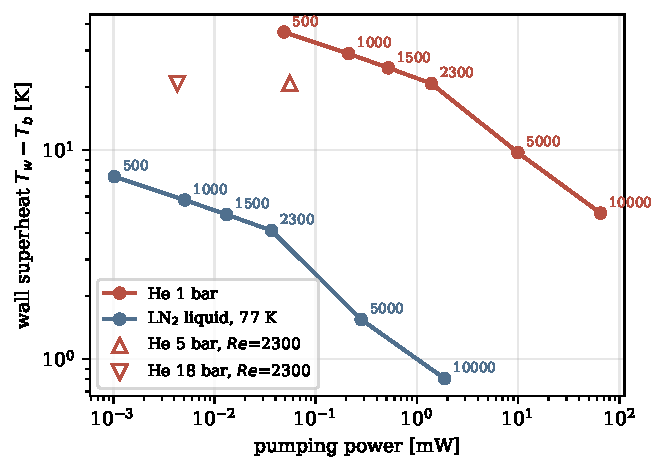
\includegraphics[width=0.75\textwidth]{fig7_pareto}
\caption{Wall superheat against pumping power for both fluids over the Reynolds sweep
(labels: $\Re$), with the helium pressure series at $\Re=2300$.}
\label{fig:pareto}
\end{figure}

\subsection{Buoyancy sensitivity}
\label{sec:res-q2-buoy}

The buoyancy parameter $\mathrm{Gr}/\Re^2$ of the forced-convection runs is at most 0.63 for
helium at 1\,bar ($\Re=500$) and above unity for nitrogen in the laminar range (40 at $\Re=500$,
1.0 at 2300), so a real plate in which gravity acts along the heated wall would carry a
mixed-convection secondary flow in nitrogen; for helium only the dense 18\,bar loop is
affected ($\mathrm{Gr}/\Re^2=7.3$ at $\Re=2300$). The four gravity-on runs confirm this.
Helium converged and gained 27\,\% in $\Nu$ at $\Re=2300$ and 118\,\% at $\Re=500$. Nitrogen
reached no steady state at either Reynolds number: after 10\,000 iterations the temperature
residual oscillated at $10^{-3}$ and the energy balance stayed open by 11\,\% and 72\,\%, the
signature of an unsteady buoyant flow a steady solver cannot represent. The forced-convection
nitrogen results therefore describe a plate with gravity normal to the heated wall or absent;
with gravity along the wall the steady model gives no bound in either direction, and the
ranking of Section~\ref{sec:res-q2-bases} is stated for forced convection only.

% =====================================================================
\section{Results Q3: the work ledger}
\label{sec:res-q3}

Table~\ref{tab:ledger} and Fig.~\ref{fig:ledger} price the two routes with
Eq.~(\ref{eq:ledger}). With ideal multipliers and the bare shield the nitrogen route is
cheaper: 37.3 against 47.4\,W, a margin of 21\,\%, because intercepting 8.3\,W at a multiplier
of 2.9 instead of 5.0 saves 18\,W while the 4\,K-stage penalty costs 7.9\,W. The emissivity
band (31.8--49.2\,W against 37.8--68.0\,W) does not close the gap. With the MLI-equivalent
shield the first-stage load shrinks to 2.6--2.7\,W, the nitrogen saving to 5.9\,W, and the verdict
flips: helium 19.0\,W against nitrogen 21.0\,W. The ideal ledger therefore favours nitrogen
where the first-stage load is large and helium where insulation has removed it, which is the
regime of the MLI-wrapped shields surveyed by Shu et al.~\cite{Shu2024AdvancedCryostats} and of the
single-layer intercepts of Singh et al.~\cite{Singh2025CryostatThermalProtection}.

With hardware efficiencies, and the shields at their nominal temperatures, the verdict is not
close in either case. The 4\,K stage at 0.8--1.5\,\% of Carnot turns the 106\,mW penalty into
520--980\,W, more than the whole first-stage bill of either route; the helium route costs
840\,W (640--1100) against 1300\,W (960--1770) for nitrogen with the bare shield and 610
against 1240\,W with MLI. The nitrogen first-stage term is not a cryocooler but the
liquefaction energy of the liquid evaporated, 0.5--0.7\,kWh\,kg$^{-1}$ against a latent heat
of 199\,kJ\,kg$^{-1}$, or $M_{\mathrm{N_2}}=9.1$--12.7\,W of plant input per watt intercepted
(a fraction-of-Carnot basis for an 80\,K cooler, 7.2--9.7, would lower the nitrogen figures by
1--2\,\%); the 4\,K-stage term is the same cryocooler stage on both routes. Written as a
break-even, the nitrogen route is cheaper only if
\begin{equation}
\frac{\eta_2}{\eta_1}\gtrsim\frac{74\,\Delta\dot Q_2}{5.0\,\dot Q_{1,\mathrm{He}}-M_{\mathrm{N_2}}\,\dot Q_{1,\mathrm{N_2}}\,\eta_1},
\label{eq:breakeven}
\end{equation}
which with the present loads and the midpoints $\eta_1=0.12$ and $M_{\mathrm{N_2}}=10.7$
requires a 4\,K-stage efficiency of 3.0\,\% of Carnot for the bare shield and 9\,\% for the
MLI shield, two to ten times what commercial coolers achieve~\cite{Radebaugh2009Cryocoolers}.
The lever is $\Delta\dot Q_2$: because 86\,\% of it is harness conduction, a harness that cuts
the 77\,$\to$\,4\,K conduction penalty threefold, by heat-sinking the drive and flux bundles
or by lower-conductivity outer conductors, brings the bare-shield break-even to 1.3\,\% of
Carnot, within the range of real hardware.

\paragraph{Coupled operating points.} The ledger above holds each shield at its nominal
temperature, but Section~\ref{sec:res-q2-maps} shows that neither cold plate sits there: the
helium plate averages 67\,K at $\Re=2300$ and reaches 50\,K only at $\Re=10^4$; the nitrogen
plate averages 81.2\,K at $\Re=2300$ and 77.8\,K at $10^4$, 4.2 and 0.8\,K above the bath,
because the duty must cross the wall superheat. The harness is heat-sunk at the plate, so the
4\,K-stage load follows the plate temperature. Table~\ref{tab:coupled} re-evaluates the ledger
with the first-stage temperature set to the area-mean plate temperature at four operating
points, using the harness integral behind Eq.~(\ref{eq:keff}) and the $T_1^4$ scaling of the
residual radiation, both reproduced by the enclosure model to 0.5\,\%, with the helium pumping
power charged at a 50\,\% circulator efficiency. At matched laminar flow the helium plate's
67\,K costs 62\,mW at the 4\,K stage and the nitrogen plate's 81\,K costs 21\,mW, and helium's
hardware advantage shrinks from 36 to 13\,\% (bare) and from 51 to 26\,\% (MLI). With each
route at the flow its design implies, helium turbulent at $\Re=10^4$ to hold 50\,K and
nitrogen laminar at $\Re=2300$, the advantage is 41 and 56\,\%; with both turbulent, 36 and
52\,\%. The ideal ledger moves the other way: at matched laminar flow nitrogen is cheaper by
25\,\% (bare) and 4\,\% (MLI). These are equivalent room-temperature powers under the stated
efficiencies and supply energies, not measured consumption; they establish the sign and order
of the difference, and that helium's advantage exists only where its plate is actually held
near 50\,K, which the flow rate, not the coolant, decides.

\begin{table}[tbp]
\centering\footnotesize\setlength{\tabcolsep}{3.5pt}
\caption{Work ledger at coupled operating points: first-stage temperature $T_1$ equal to the
area-mean plate temperature of the cold-plate model (He at 1\,bar; 18\,bar changes only the
negligible pumping term); $\dot Q_2$ from the harness integral and the scaled residual
radiation; equivalent room-temperature power with ideal multipliers and with mid-range
hardware efficiencies (ranges in \texttt{data/ledger\_coupled.csv}).}
\label{tab:coupled}
\begin{tabular}{l r r r r r}
\toprule
Operating point (He / \LNtwo) & $T_1$ [K] & $\dot Q_2$ [mW] & $\dot W_{\mathrm{ideal}}$ [W] & $\dot W_{\mathrm{real}}$ [W] & He advantage, real \\
\midrule
\multicolumn{6}{l}{\textit{bare shield}} \\
nominal, decoupled & 50 / 77 & 73 / 180 & 47.4 / 37.3 & 840 / 1300 & 36\,\% \\
matched $\Re=2300$, both laminar & 67.1 / 81.2 & 135 / 201 & 51.7 / 38.8 & 1250 / 1450 & 13\,\% \\
own design points: He $\Re=10^4$, \LNtwo\ $\Re=2300$ & 50.3 / 81.2 & 74 / 201 & 47.5 / 38.8 & 850 / 1450 & 41\,\% \\
both turbulent, $\Re=10^4$ & 50.3 / 77.8 & 74 / 184 & 47.5 / 37.6 & 850 / 1330 & 36\,\% \\
\addlinespace[2pt]
\multicolumn{6}{l}{\textit{MLI-equivalent shield}} \\
nominal, decoupled & 50 / 77 & 73 / 180 & 19.0 / 21.0 & 610 / 1240 & 51\,\% \\
matched $\Re=2300$, both laminar & 67.1 / 81.2 & 135 / 201 & 23.4 / 22.5 & 1020 / 1380 & 26\,\% \\
own design points & 50.3 / 81.2 & 74 / 201 & 19.1 / 22.5 & 610 / 1380 & 56\,\% \\
both turbulent, $\Re=10^4$ & 50.3 / 77.8 & 74 / 184 & 19.1 / 21.3 & 610 / 1270 & 52\,\% \\
\bottomrule
\end{tabular}
\end{table}

\begin{table}[tbp]
\centering\small
\caption{Work ledger at the nominal shield temperatures: stage loads (row-normalised view
factors) and equivalent room-temperature power, ideal and hardware-based. Ranges: emissivity $\pm50$\,\% (ideal) and the stage-efficiency and
nitrogen supply-energy ranges of Supplementary Table~S9 (real).}
\label{tab:ledger}
\begin{tabular}{l l r r r r}
\toprule
Shield & Route & $\dot Q_1$ [W] & $\dot Q_2$ [mW] & $\dot W_{\mathrm{ideal}}$ [W] & $\dot W_{\mathrm{real}}$ [W] \\
\midrule
bare & He, 50\,K & 8.39 & 73.5 & 47.4 (37.8--68.0) & 840 (640--1100) \\
bare & \LNtwo, 77\,K & 8.30 & 179.9 & 37.3 (31.8--49.2) & 1300 (960--1770) \\
MLI-eq. & He, 50\,K & 2.72 & 73.5 & 19.0 & 610 (450--820) \\
MLI-eq. & \LNtwo, 77\,K & 2.65 & 179.9 & 21.0 & 1240 (910--1700) \\
\bottomrule
\end{tabular}
\end{table}

\begin{figure}[tbp]
\centering
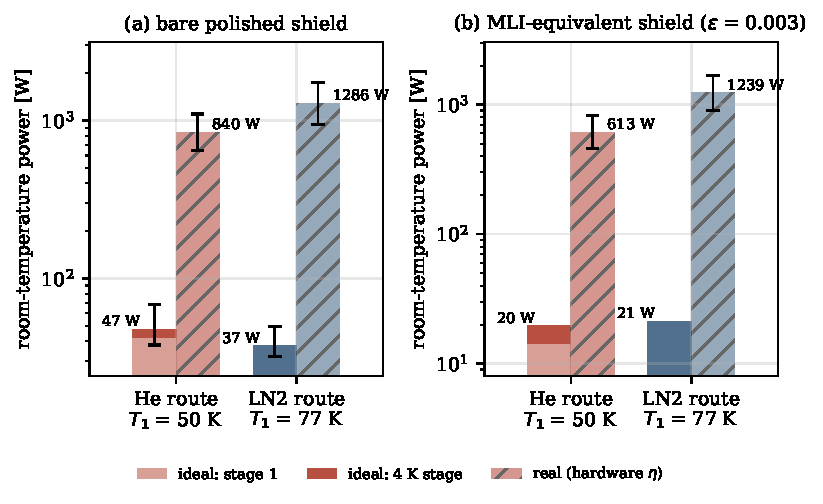
\includegraphics[width=\textwidth]{fig8_ledger}
\caption{Room-temperature power of the two routes for (a)~the bare polished shield and
(b)~the MLI-equivalent shield: ideal Carnot multipliers split by stage (solid) and hardware
efficiencies (hatched), with emissivity and efficiency ranges as error bars.}
\label{fig:ledger}
\end{figure}

% =====================================================================
\section{Discussion}
\label{sec:discussion}

\paragraph{The penalty is a harness property.} The passive cost of the warmer shield is
located, sized and attributed: 106\,mW at the 4\,K stage, 86\,\% of it conduction along a
harness whose drive and flux families carry three quarters. It is a property of the wiring,
not of the cryogen, and Eq.~(\ref{eq:breakeven}) shows that, at the efficiencies of present
hardware, the wiring is the variable that moves the break-even most. Lumped budgets give the same
total, and its split among bundles follows from the cable counts; what the resolved model
adds is the coupling of the harness to the radiation field, the flux distribution over the
shield, the closure behaviour of the view-factor matrix, the confirmation that the residual
radiation is a minor term at any shield temperature, and the dependence of the 4\,K load on
the plate temperature that the coupled ledger of Table~\ref{tab:coupled} uses. This is the design steer that Li et al.'s optimisation of intercepts on supports and in
insulation~\cite{Li1990SMESIntercepts} cannot give for a wired cryostat.

\paragraph{The helium plate floats.} A cold plate cooled by circulated helium gas at
atmospheric pressure does not sit at the gas temperature. At the 9.4\,W duty it runs 21\,K
above the bulk at $\Re=2300$, with a hottest face 13\,K above that mean; the mean reaches
nitrogen temperature at $\Re\approx970$ and the hottest face only at $\Re\gtrsim2300$, and the
nominal 50\,K is approached only at $\Re=10^4$ and tens of milliwatts of pumping power.
Pressurising the loop leaves the wall temperature untouched but makes the pumping power
negligible. This concerns the circulated-gas architecture, not the conductively coupled PTR
first stage of Fig.~\ref{fig:schematic}a, whose plate temperature is set by the cooler's
capacity curve. The 50/77\,K distinction of the passive comparison is therefore realised on
the helium route only with adequate flow or pressure (Section~\ref{sec:res-q2-maps}).

\paragraph{The three questions couple through the plate temperature.} The ledger credits the
helium route with a 50\,K shield, but the cold plate reaches 50\,K only at $\Re\approx10^4$;
at the laminar design point of $\Re=2300$ and 1\,bar its mean is 67\,K, where the harness
integral of Eq.~(\ref{eq:keff}) gives a 4\,K-stage conduction of 125\,mW against 70\,mW at
50\,K and 162\,mW at 77\,K. A helium shield run there forfeits 54\,mW, 59\,\% of the 92\,mW
conduction penalty that separates the routes, and about 4\,W of the 7.9\,W ideal advantage;
the 65\,mW of pumping power that buys the 50\,K plate at $\Re=10^4$ is negligible against
that, so on the helium route the flow rate is set by the 4\,K ledger. The nitrogen plate is
not pinned by the bath either: it sits 4.2\,K above it at $\Re=2300$ and 0.8\,K at $10^4$,
worth 21 and 4\,mW at the 4\,K stage, a smaller and flow-insensitive coupling because the
liquid's superheat is small. Table~\ref{tab:coupled} carries both into the ledger; what
remains of the bath-pinning idea is a plate temperature that the flow rate barely moves.

\paragraph{The basis of comparison decides the ranking.} Matched Reynolds number, matched mass
flow and matched pumping power rank the fluids differently in magnitude and, for pumping
power at 18\,bar, in sign. The effectiveness--NTU pair inverts the engineering conclusion
because it rewards a small capacity rate. A cryogenic coolant comparison must therefore state
its basis and its operating point, as Gačnik et al.\ found necessary for nitrogen-cooled
terminals~\cite{Gacnik2025LN2Terminals}; the operating maps of Fig.~\ref{fig:maps} are offered
as the form such a comparison should take.

\paragraph{Ideal and real ledgers disagree, and the disagreement is informative.} The ideal
ledger prefers nitrogen for a bare shield and helium for an insulated one; the hardware
ledger prefers helium in both cases, by 36--51\,\% at the nominal shield temperatures and by
13--56\,\% at the coupled operating points of Table~\ref{tab:coupled}, because the 4\,K
stage of a commercial cooler converts each milliwatt of penalty into 5--9\,W at the wall. The nitrogen route
retains what Li et al.\ identified three decades ago~\cite{Li1990SMESIntercepts}: a constant
shield temperature, stored reserve, and independence from the cryocooler, which now also
means freedom from its vibration~\cite{Tomaru2004Vibration}. Those are operational
arguments; the thermodynamic one is conditional on the harness.

\paragraph{Methodological findings.} Two travel beyond this geometry. First, view-factor
matrices generated for low-emissivity enclosures must be checked for closure and, if the
enclosure is closed, row-normalised, which restores closure though not reciprocity; the
required closure accuracy is of order the emissivity, and agglomeration refinement does not
supply it, whereas the normalised load converges under it. The benchmark practice of
Končar et al.~\cite{Koncar2018CFDRadiation} should be extended by this test. Second, the
mixing-cup temperature on a graded mesh must be mass-flux weighted without an additional
area factor; the corrected accounting closed the energy balance of every run from a few per
cent to below 0.2\,\%.

\paragraph{Limitations.} The enclosure imposes fixed temperatures on its plates and shield and
neglects contact resistance at the harness ends; a finitely conductive shield would carry the
radiative-flux map of Fig.~\ref{fig:fields} into a temperature map, which is the next step.
The cold plate is a single-wall-heated smooth duct with constant properties except for the
helium density and the nitrogen buoyancy term; conjugate conduction in the plate, which would
spread the wall temperature, is not resolved. Nitrogen is single phase by verified margin at
3\,bar but not at 1\,bar. The turbulent runs rely on the SST model at $y^+\le 9.5$ and were
not compared with experiment. The hardware efficiencies are survey ranges, with the two-stage cooler's efficiency split
between stages from those ranges rather than from one machine; a measured capacity map would
replace them. Nitrogen buoyancy was shown to be unsteady and excluded from the ranking rather
than resolved; a transient calculation in a specified plate orientation would quantify it.

% =====================================================================
\section{Conclusions}
\label{sec:conclusions}

\begin{enumerate}
\item A 77\,K first shield costs essentially nothing at the first stage relative to a 50\,K
shield: 99.6\,\% of the radiation and 6.5\,\% less harness conduction, 8.3 against 8.4\,W. The
penalty appears at the 4\,K stage, 106\,mW, 86\,\% of it harness conduction in the drive and
flux bundles, worth 7.9\,W of ideal room-temperature power and 520--980\,W with real 4\,K
coolers.
\item View-factor radiation in low-emissivity enclosures is controlled by matrix closure: the
generated matrix gave 9.5 to 3.3\,W under agglomeration refinement against a 7.07\,W closed
form; row normalisation recovers it to 4\,\% at the first stage and 0.5\,\% at the 4\,K stage
and converges under refinement (7.36, 7.32, 7.27\,W at 250, 400, 800 faces).
\item As a first-shield coolant at 9.4\,W, nitrogen gives 5 times helium's heat-transfer
coefficient in laminar flow and 6 in turbulent flow and holds the plate within about 4\,K of
its inlet at $\Re=2300$ against helium's 21\,K; helium at 1\,bar lets the plate mean float
above 77\,K below $\Re\approx970$ and its hottest face above 77\,K in every constant-property
laminar run (76.9\,K at $\Re=2300$ with variable properties) and needs 38 times the pumping
power, but at 18\,bar its pumping power falls below nitrogen's by 8.5 times with heat transfer
unchanged. At each fluid's optimum nitrogen needs 1.0\,$\mu$W at $\Re=500$; helium at 18\,bar
needs 0.6\,$\mu$W on the plate-mean criterion and 4 to 31\,$\mu$W on the hottest-face
criterion. The ranking depends on the basis, the operating point and the wall criterion.
\item The ideal ledger favours nitrogen by 21\,\% for a bare shield and helium by 9\,\% with
MLI; with hardware efficiencies and the liquefaction energy of the nitrogen consumed, the
equivalent room-temperature power favours helium by 36--51\,\% at the nominal shield
temperatures and by 13--56\,\% at the coupled operating points, an advantage that exists only
where the helium plate is actually held near 50\,K. Nitrogen becomes competitive when the
77\,$\to$\,4\,K harness conduction is cut by about a factor of three, the lever of
Eq.~(\ref{eq:breakeven}).
\item The comparison rests on code-verified numbers: NIST properties at a stated reference
state, a forced-convection basis with gravity-on sensitivity, a mass-flux-weighted mixing-cup
temperature closing the energy balance to 0.2\,\%, wall temperatures read from the wall
itself, and row-normalised view factors reproducing the closed forms to 4\,\%. That the shield
choice and the harness design are not separable follows from those numbers; experimental
validation of the cold-plate model is the next step.
\end{enumerate}

\section*{CRediT authorship contribution statement}
\textbf{Imerson Joao:} Conceptualization, Methodology, Software, Investigation, Formal
analysis, Visualization, Writing -- original draft, Writing -- review \& editing.

\section*{Declaration of competing interest}
The author declares no known competing financial interests or personal relationships that
could have influenced the work reported in this paper.

\section*{Data availability}
All OpenFOAM cases (enclosure baseline and variants, cold-plate sweep, grid studies), the
post-processing and figure scripts, and the tabulated results are available at
\\ \noindent{\footnotesize\href{https://github.com/Imerson/cryostat-first-shield-He-vs-LN2}{github.com/Imerson/cryostat-first-shield-He-vs-LN2}}; an archived copy will be deposited on Zenodo on acceptance.

\section*{Acknowledgements}
The author thanks Dr.\ Konstantina Vogiatzaki and Dr.\ Natalia Ares for supervision and
discussions.

\section*{Declaration of generative AI in scientific writing}
During the preparation of this work the author used Claude (Anthropic) to assist with
editing, revision and consistency checking of the manuscript and with scripting the
simulation campaign. The author reviewed and edited all content and takes full
responsibility for the published article.

\bibliographystyle{elsarticle-num}
\bibliography{precooling_refs}
\end{document}
